\documentclass[11pt]{article}

%\usepackage[spanish,es-lcroman]{babel}
\usepackage[spanish]{babel}
\usepackage[utf8]{inputenc}
\usepackage{amsmath, amsthm, amssymb}
\usepackage{graphicx} % fugures
\usepackage{wrapfig} %figuras con texto al lado
\usepackage{float} 
\usepackage{siunitx}
\usepackage{mathrsfs}
\usepackage{parskip} % remove the indent 
\usepackage{empheq} % close equations with align in a box / for one eq. to use only \boxed
\usepackage[none]{hyphenat} % for latex does not cut the words 

\decimalpoint 

\title{Cosmología. Marco Teórico}
\author{Margionet Díaz}
\date{December 2018}

\begin{document}

\sloppy % las corta pero justifica el párrafo 

\numberwithin{equation}{section} % enurate equations by section 

\maketitle

\section{Principio Cosmológico}

La isotropía de la Radiación del Fondo Cósmico de Microondas (CMB) nos dice que a primera aproximación el Universo es isotrópico y homogéneo actualmente. Esto último fue asumido en 1917 por Einstein en su modelo estático, que sería el primer modelo del Universo autoconsistente (Einstein, 1917). También, los modelos de Friedman tiempo después se convertirían en los modelos estándar para las dinámicas a gran escala del Universo y eran basados en soluciones de expansión de las ecuaciones de Einstein siguiendo las pistas de de Sitter y Lanczos.



Con respecto a las coordenadas del espacio y tiempo utilizadas, en 1923 Hermann Weyl introdujo su ``Postulado de Weyl'' (Weyl, 1923) que establecía la noción de geodésicas divergentes, las cuales representan las líneas de mundo de galaxias, que no se intersectan excepto en un punto singular del pasado finito o infinito. Según esto, existe sola una geodésica pasando a través de cada punto en el espacio-tiempo, excepto en el origen.  De aquí es posible asignar un observador a cada línea de mundo. A esto se le conoce como {\textit{Observadores fundamentales}} donde cada uno de ellos lleva un reloj estándar y el tiempo medido en ese reloj desde el punto singular se llama {\textit{tiempo cósmico}}.

En 1935 Robertson y Walker (Robertson, 1935; Walker, 1936) derivaron la métrica del espacio-tiempo para todos los modelos de Universos isotrópicos, homogéneos y en expansión uniforme la cual era independiente de la suposición de que las dinámicas a gran escala eran descritas por la Teoría de la Relativdad General, i.e., no importaba cual fuera la física de la expansión,  la forma de la métrica era la de Robertson - Walker, esto partiendo del supuesto de isotropía y homogeneidad del Universo. 

Otra consideración para construir un modelo cosmológico es el conocido {\bf{principio cosmológico}} de donde podemos afirmar que: ``no estamos ubicados en ningún lugar especial en el Universo'', no hay preferencia, por lo que cualquier observador fundamental ubicado en cualquier lugar del Universo pero en la misma época cósmica observa las mismas características a grande escala que nosotros, i.e., la misma expansión de Hubble de la distribución de galaxias, la misma radiación del CMB isotrópica, la misma estructura esponjosa a gran escala de la distribución de galaxias y vacíos (red cósmica), y así sucesivamente. 
En un sistema de galaxias que se expanden, cada observador en cada galaxia individual observa el mismo flujo de Hubble en la misma época, así, todos tienen derecho a creer que son el centro de un Universo en expansión. 

En cuanto a la geometría, a finales del siglo XVIII se estaban considerando los espacios no euclidianos. Los padres de la geomtría no euclidiana Nikolai Ivanovich Lobachevsky en Rusia y János Bolyai en Transilvania (Lobachevsky, 1829; Bolyai, 1830). Lobachevsky resolvió el problema de la existencia de geometrías no euclidianas, así la misma se puso sobre una base teórica sólida por los estudios de Bernhard Riemann. 

 \begin{wrapfigure}{r}{0.4\linewidth}          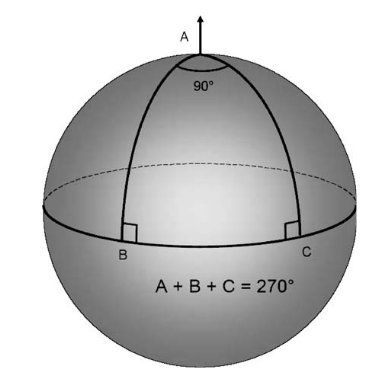
\includegraphics[width=0.5\textwidth]{superficie_esferica_pp152.png}
    \caption{\footnotesize{Suma de los ángulos de un triángulo en la superficie de una esfera}}
    \end{wrapfigure}
    
A través de la geometría riemanniana, Einstein fue capaz de combinar la relatividad especial con la teoría de la gravedad y el cálculo tensorial, lo que fue un logro monumental de la época. Fue así como Einstein se dio cuenta que tenía las herramientas necesarias con las que podría construir modelos totalmente coherentes del Universo, donde su propuesta era un Universo estático, cerrado y con geometría esférica isotrópica. Por otro lado, los modelos de Friedman eran también modelos isotrópicos pero con soluciones de expansión que incluían geometrías que eran tanto esféricas como hiperbólicas (Friedman, 1922, 1924). 

En la figura 1 se tiene el caso más simple de la geometría curvada en 2 dimensiones, la superficie de una esfera: un triángulo con dos líneas (con $90^{\circ}$ entre ellas) que parten del polo norte y llegan hasta el ecuador, y una tercera línea que se dibuja sobre el ecuador. Estas líneas son la distancia más corta entre entre las tres esquinas del triángulo. En geometría curva son geodésicas. 

De fig. 1, si el radio de una esfera es $R_c$, el área superficial del triángulo ABC es $A= \theta R_c$ y variando el ángulo se obtiene para $\theta = 90^{\circ} \rightarrow{A = \pi R_c^2/2}$ y la suma de los ángulos del triángulo es $270º$ y si $\theta=0º$ entonces el área es cero y la suma de los ángulos $180º$. Así, la diferencia de la suma de los ángulos de $180º$ es proporcional al área del triángulo:
$$(\text{suma de los ángulos del triángulo} - 180º \propto \text{área del triángulo},$$
la cual es una propiedad general de los espacios curvos isotrópicos. 

   \vspace{0.5cm}

\subsection{La métrica espacio-tiempo para espacios isotrópicos curvos}

\begin{equation}
  dl^2 = dx^2 + dy^2 + dz^2,  
\end{equation}
Representa la distancia entre dos puntos separados por $dx, dy, dz$ en un espacio plano. 

Siendo el caso más simple de un espacio curvo bidimensional isotrópico la superficie de una esfera, es conveniente utilizar un sistema coordenado polar para describir posiciones en la superficie (ver figura 1) que para el caso, las coordenadas ortogonales son $\theta$ y $\phi$ y el aumento de la distancia $dl$ entre dos puntos en dicha superficie es:

\begin{equation}
    dl^2 = R_c^2 d\theta^2 + R_c^2 \sin^2 \theta d\phi^2,
\end{equation}

    donde $R_c$ es el radio de curvatura de la superficie del espacio bidimensional, para el caso, el radio de la esfera. (2) es la {\textit{métrica de la superficie bidimensional}} y puede generalizarse como:
    
    \begin{equation}
        dl^2 = g_{\mu \nu} dx^{\mu} dx^{\nu}, 
    \end{equation}
    
    siendo el {\textit{tensor métrico}} el contenedor de toda la información acerca de la geometría intrínseca del espacio. Otros sistemas de coordenadas pueden definir las coordenadas de un punto en cualquier superficie bidimensional. Para un plano euclidiano: 

\begin{equation}
    dl^2 = dx^2 +  dy^2,
\end{equation}

en polares

\begin{equation}
    dl^2 = dr^2 + r^2 d\phi^2.
\end{equation}

Con el tensor métrico $g_{\mu \nu}$ es posible determinar la curvatura intrínseca del espacio, y esto fue probado por Gauss. Para tensores que pueden ser reducidos a la forma diagonal (ecs. 2, 4, 5) la curvatura intrínseca viene dada por:


    \begin{align*}
        \kappa & = \frac{1}{2 g_{11} g_{22}} \left\{ - \frac{\partial^2g_{11} }{\partial x_2^2} - \frac{\partial^2g_{22} }{\partial x_1^2} + \frac{1}{2 g_{11}} \left[ \frac{\partial g_{11} }{\partial x_1} \frac{\partial g_{22} }{\partial x_1} +   \left( \frac{\partial g_{11} }{\partial x_2} \right)^2 \right] 
        + \frac{1}{2 g_{22}} \left[ \frac{\partial g_{11} }{\partial x_2} \frac{\partial g_{22} }{\partial x_2} + \left( \frac{\partial g_{22} }{\partial x_1} \right)^2 \right] \right\} 
    \end{align*}

$\kappa$ se conoce como la {\textit{curvatura gaussiana}} del bi-espacio. La extención a tres espacios isotrópicos es sencilla si mantenemos que cualquier sección bidimensional a través de un espacio tridimensional isotrópico debe ser un bi-espacio isotrópico y ya el tensor métrico par este caso es conocido. 

Fue mencionado que para un bi-espacio isotrópico, las coordenadas adecuadas son las polares esféricas. De la fig. 2, la distancia alrededor del arco de un gran círculo desde el punto $O$ hasta $P$ es $R_c \theta$, por lo que la métrica se escribe:

    \begin{equation}
        dl^2 = d\varrho^2 + R_c^2 \sin^2\left(\frac{\varrho}{R_c} \right) d\phi^2,
    \end{equation}

donde $\varrho$ es la distancia más corta entre $0-P$  en la superficie de una esfera ya que es parte de un gran  círculo. De esta manera, estamos hablando de una {\textit{distancia geodésica}} en el espacio curvo isotrópico. Recordemos que en espacios curvos las geodésicas juegan el rol de las líneas rectas.

    \begin{wrapfigure}{r}{0.5\linewidth}               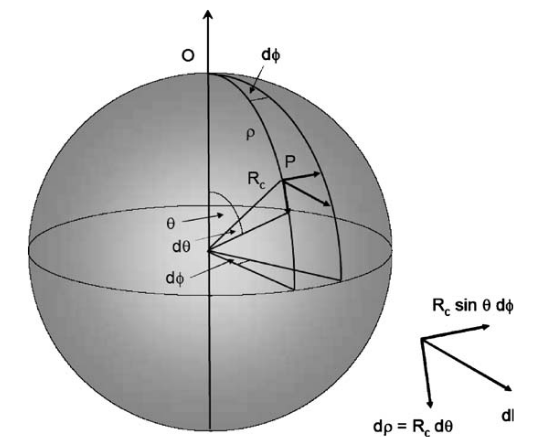
\includegraphics[width=0.5\textwidth]{superficie_esferica_pp156_angulos.png}
        \caption{\footnotesize{$\varrho$ es la distancia radial alrededor de la esfera desde el polo y el ángulo $\phi$ mide los desplazamientos angulares en el polo.}}
    \end{wrapfigure}

Ahora, (6) puede ser reescrita como: 

    \begin{equation}
        x = R_c \sin \left(\frac{\varrho}{R_c} \right).
    \end{equation}
    
    Hallando $dx^2$ con $$d\varrho^2 = \frac{dx^2}{1-\kappa x^2},$$
    la métrica puede ser escrita como: 
    
    \begin{equation}
        dl^2 = \frac{dx^2}{1-\kappa x^2} + x^2d\phi^2.
    \end{equation}
    
    \vspace{0.6cm}
    Recordando que $\kappa = 1/R_c^2$, tres casos deben ser considerados: 
    
    \begin{equation*}
     \label{eq:aqui-le-mostramos-como-hacerle-la-llave-grande}
     \kappa  = \left\{
	       \begin{array}{ll}
		 > 0      & {\text{espacio esférico}},, \\
		 = 0 & R_c \rightarrow{\infty}, \hspace{0.4cm}  {\text{espacio plano}}, \\
		 < 0     & {\text{espacio hiperbólico}}.
	       \end{array}
	     \right.
   \end{equation*}
    
    \vspace{0.4cm}
    
Para $\kappa = 0$ se recupera el espacio euclidiano.

Para el incremento espacial en un espacio tridimensional curvo recordemos que cualquier sección bidimensional a través de un tri-espacio isotrópico debe ser un espacio isotrópico de dos dimensiones donde la métrica puede ser ec. (6) o (8). En coordenadas polares esféricas, el desplazamiento angular general perpendicular a la dirección radial es 
\begin{equation}
    d\phi^2 = d\theta^2 +  \sin^2 \theta d\phi^2.
\end{equation}
 (con $\theta$ y $\phi$ diferentes a los usados en la figura 2). De esta manera, se puede escribir el incremento espacial (de 6 y 8) 


\begin{align}
        dl^2 & = d\varrho^2 + R_c^2 \sin^2\left(\frac{\varrho}{R_c} \right) [d\theta^2 +  \sin^2 \theta d\phi^2], \\
        dl^2 &  =  \frac{dx^2}{1-\kappa x^2} + x^2[d\theta^2 +  \sin^2 \theta d\phi^2].
\end{align}

De esta manera, la {\textit{métrica de Minkowski}} para un tri-espacio isotrópico viene escrita como: 

\begin{equation}
    ds^2 = dt^2 - \frac{1}{c^2} dl^2,
\end{equation}

con $dl$ el de las expresiones (10) u (11). Aunque $x$ y $\varrho$ son medidas de distancias equivalente, su significado físico es bastante distinto. A continuación, podemos derivar la métrica de Robertson -  Walker. 


\subsection{Métrica de Robertson - Walker}

Queremos aplicar la métrica de Minkowski, ec. 12, a modelos de mundo homogéneos, isotrópicos. Para eso, debemos recurrir a:

    \begin{enumerate}
        \item Principio cosmológico: A primera aproximación, el Universo es isotrópico y homogéneo en la época actual.
        \item Observadores fundamentales: quienes se mueven de modo tal que el Universo siempre parece isotrópico para ellos. 
        \item Tiempo cósmico: cada uno de estos observadores lleva un reloj y el tiempo propio medido por ese reloj es lo que se conoce como {\textit{tiempo cósmico}}.
    \end{enumerate}
    
Recordemos que según el postulado de Weyl, las geodésicas de todos los observadores se reunen en un punto en el pasado y el tiempo cósmico puede ser medido desde esa época de referencia. 

Ahora bien, considerando las ecs. 10 y 12, podemos escribir la métrica como:

    \begin{equation}
        ds^2 = dt^2 - \frac{1}{c^2}( d\varrho^2 + R_c^2 \sin^2\left(\frac{\varrho}{R_c} \right) (d\theta^2 +  \sin^2 \theta d\phi^2)],
    \end{equation}

siendo $t$ el tiempo cósmico y $d\varrho$ un incremento de la distancia propia en la dirección radial. 

Para un Universo en expansión, esta métrica presenta problemas. Ya que la luz viaja una velocidad finita, observamos todos los objetos astronómicos a lo largo de un cono de luz anterior centrado en la Tierra en la época actua $t_0$ (ver figura 3). Así, cuando observamos objetos distantes, no los observamos en la época actual sino en un tiempo anterior $t_1$, cuando el Universo todavía era homogéneo e isotrópico, pero las distancias entre los fundamentales eran menores y la curvatura espacio diferente. Significa entonces que la métrica 13 solo puede ser aplicada a un espacio curvo, isotrópico definido en una única época. 

\begin{wrapfigure}{r}{0.5\linewidth}               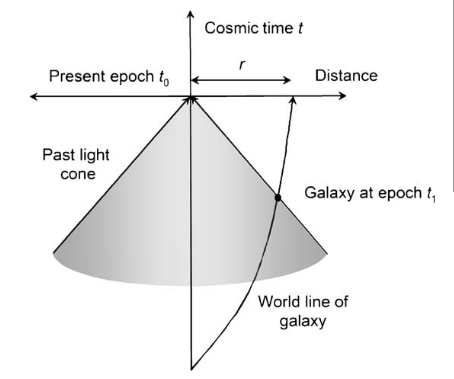
\includegraphics[width=0.65\textwidth]{cono_luz_pp159.png}
        \caption{\footnotesize{Diagrama de espacio-tiempo que ilustra la definición de la distancia de la coordenada radial comovil.}}
    \end{wrapfigure}
    
    
Para medir una distancia propia adecuada que pueda ser incluida en (13)  se pueden alinear un conjunto de observadores fundamentales que estén entre la Tierra y la galaxia. Cada uno de estos observadores va a medir la distancia $d \varrho$ a su próximo observador en un tiempo cósmico particular. Al sumar todos estos $d \varrho$ se puede obtener una distancia adecuada que es medida en una sola época y con la que sería posible incluir en la métrica (13). Lo que nosotros observamos son galaxias distantes en una época pasada, i.e., cómo eran en una época anterior, y no se sabe cómo proyectar sus posiciones relativas a nosotros en la época actual hasta que conozcamos la cinemática del Universo en expansión. Es por esto que la distancia depende de la elección del modelo cosmológico que se considere. 

En una expansión uniforme la distancia entre dos observadores fundamentales, $i,j$ en dos épocas $t_1$ y $t_2$ cambia de manera que 

    \begin{align}
        \frac{\varrho_i(t_1)}{\varrho_j(t_1)} & = \frac{\varrho_i(t_2)}{\varrho_j(t_2)} = {\text{constante}} \notag \\
        \frac{\varrho_i(t_1)}{\varrho_i(t_2)} & = \frac{\varrho_j(t_2)}{\varrho_j(t_2)} = ... =  {\text{constante}} = \frac{a(t_1)}{a(t_2)}.
    \end{align}


En modelos isotrópicos, $a(t)$ representa una función universal conocida como {\bf{factor de escala}}, la cual explica cómo la distancia entre cualquiera de los dos observadores fundamentales cambia con el tiempo cósmico $t$. 
Si tomamos $a(t) = 1$ para la época presente, $t_0$, y renombramos el valor de $\varrho$ en el presente como $r$, (14) se escribe como

    \begin{equation}
        \varrho (t) = a(t)r,
    \end{equation}

donde $r$ lleva la etiqueta de distancia, la cual está unida a una galaxia u observador fundamental durante todo el tiempo y recibe el nombre de {\bf{coordenada de distancia radial comóvil}}. La variación en la distancia propia en el Universo en expasión es $a(t)$. Las distancias propias perpendicular a la línea de visión también pueden cambiar por un factor $a$ entre $t_0$ y $t$, a causa de la isotropía de y homogeniedad del modelo, 

\begin{equation}
    \frac{\Delta l(t)}{\Delta l(t_0)} = a(t).
\end{equation}

De la métrica (13) 

    \begin{align}
        a(t) & = \frac{R_c(t) \sin[\varrho/R_c(t)] d \theta}{R_c(t_0) \sin[r/R_c(t_0)] d \theta}, \\
    \frac{R_c(t)}{a(t)} \sin \left[\frac{a(t)r}{R_c(t)} \right] & = R_c(t_0) \sin \left[\frac{r}        {R_c(t_0)} \right],
    \end{align}

válido siempre que 
    \begin{equation}
        R_c (t) = a(t) R_c (t_0),
    \end{equation} 

de aquí que, para conservar la isotropia y homegeindad, {\bf{la curvatura del espacio cambia a medida que el Universo se expande}} como $k = R_c^{-2} \propto a^{-2}$. 

Si ahora el radio de curvatura de la geometría del espacio $R_c$ en la época presente lo etiquetamos como R'
    \begin{equation}
        R_c (t) = a(t) R'.
    \end{equation}

Sustituyendo (15) y (19) en (13):

    \begin{equation}
        ds^2 = dt^2 - \frac{a^2(t)}{c^2} [dr^2 + R'^2 \sin^2(r/R')(d \theta^2 + \sin^2 \theta d\phi^2)],
    \end{equation}

obtenemos la {\bf{métrica de Robertson - Walker}}, la cual contiene dos incognitas: 

    \begin{enumerate}
        \item La función desconocida pero etiquetada como el factor de escala $a(t)$, que describe la dinámica del Universo,
        \item La constante, también desconocida, $R'$, la cual describe la curvatura espacial del Universo en la época presente. 
    \end{enumerate} 

También, si se usa la {\bf{distancia de diámetro angular comóvil}}: $r_1 = R' \sin(r/R')$, la métrica puede ser escrita como:

    \begin{equation}
        ds^2 = dt^2 - \frac{a^2(t)}{c^2} \left[ \frac{dr_1^2}{1 - \kappa r_1^2} + r_1^2 (d\theta^2 + \sin^2 \theta d\phi^2) \right],
    \end{equation}

    siendo ahora $\kappa = 1/R'^2$. Además, por un reescalamiento adecuado de la coordenada $r_1$: $\kappa r_1^2=r_2^2$, la métrica se escribe:

    \begin{equation}
        ds^2 = dt^2 - \frac{R_1^2(t)}{c^2} \left[ \frac{dr_2^2}{1 - \kappa r_2^2} + r_2^2 (d\theta^2 + \sin^2 \theta d\phi^2) \right],
    \end{equation}

donde $\kappa = +1, 0 -1$ para universos con geometría esférica, plana o hiperbólica. En este reescalamiento $R_1(t)= R_c(t_0) a= R'a$ por lo que $R_1(t)$ en la época presente es $R'$ más bien que la unidad. 
Las métricas (19), (20) y (21) pueden definirnos el intervalo invariante $ds^2$ entre eventos en cualquier época o lugar en el Universo en expansión. 

Finalmente, vamos a repasar algunos aspectos importantes:

    \begin{enumerate}

        \item El {\bf{tiempo cósmico $t$}} es el tiempo medido por un reloj llevado por el observador fundamental,
        \item {\bf{$r$ es la coordenada de distancia radial comovil}} que está fija a una galaxia para siempre y que es la distancia propia que tendría la galaxia si sus líneas de mundo fueran proyectadas hacia adelante a la época $t_0$ y sus distancias medidas en ese tiempo. 
        \item $a(t)dr$ es el {\bf{elemento de distancia propia (geodésica) en la dirección radial en la época}} $t$. 
        \item $a(t) [R'\sin(r/R')] d\theta = a(t) r_1 d\theta$ es el {\bf{elemento de distancia propia perpendicular a la dirección radial subtendida por el ángulo}} $d\theta$ en el origen. 
        \item $a(t) [R'\sin(r/R')] \sin \theta d\phi = a(t) r_1 \sin \theta d\phi$ es el {\bf{elemento de distancia propia en la dirección}} $\phi$.
        
        No sabemos nada acerca de la física que gobierna la tasa de expansión de Universo; sin embargo, $a(t)$ absorbe este fenómeno todavía desconocido.  
        
    \end{enumerate} 



\section{Observaciones en Cosmología}

\subsection{Corrimiento al Rojo Cosmológico}

Cuando hablamos del corrimiento al rojo cosmológico, nos referimos al desplazamiento de las líneas espectrales hacia longitudes de onda más grandes asociadas a la expansión isotrópica del sistema de galaxias. Así, el corrimiento al rojo $z$ es definido como

\begin{equation}
    z = \frac{\lambda_0 - \lambda_e}{\lambda_e},
\end{equation}

siendo $\lambda_0$ la longitud de onda observada y $\lambda_e$ la longitud de onda de la línea emitida.  



Si $z$ fuera interpretada como una velocidad de recesión $v$ de una galaxia, $z$ y $v$ serían relacionadas por el desplzamiento Doppler Newtoniano

    \begin{equation}
        v= cz,
    \end{equation}

que fue utilizada por Hubble para derivar la relación velocidad-distancia, $v=H_0 r$. 

En cosmología, el corrimiento al rojo tiene un significado más profundo. Por ejemplo, si consideramos un paquete de ondas de frecuencia $\nu_1$ emitido entre los tiempos cósmicos $t_1$ y $t_1 +  \Delta t_1$ de una galaxia distante, y es recibido por un observador en la época presente $t_0$ y $t_0 + \Delta t_0$, la señal se propaga a lo largo de {\bf{conos nulos}}, $ds^2=0$, y si además $d\theta = d\phi = 0$, la métrica (19) puede escribir como:

    \begin{equation}
        dt = - \frac{a(t)}{c} dr \hspace{0.4cm} \frac{c dt}{a(t)} = -dr,
    \end{equation} 

con $a(t) dr$ el {\bf{intervalo de distancia propia en el tiempo cósmico}} $t$. Para el borde delantero del paquete de ondas 

    \begin{equation}
        \int_{t_1}^{t_0} \frac{cdt}{a(t)} = - \int_r^0{dr}.
    \end{equation}
        
Y el final del paquete de ondas debe viajar la misma distancia en unidades de la coordenada de distancia comovil ya que $r$ es fija a la galaxia para siempre. Así:

    \begin{align} 
        \int_{t_1 + \Delta t_1}^{t_0 + \Delta t_0}{ \frac{cdt}{a(t)}} & = - \int_r^0{dr}, \\
        \int_{t_1}^{t_0}{ \frac{cdt}{a(t)} +  \frac{c \Delta t_0}{a(t_0)} -\frac{c \Delta t_1}{a(t_1) }}   & =  \int_{t_1}^{t_0}{ \frac{cdt}{a(t)}}. 
     \end{align}

 Y ya que $a(t_0) = 1$

    \begin{equation}
        \Delta t_0 = \frac{\Delta t_1}{a(t_1)}.
    \end{equation}


Esta es la expresión para el fenómeno de la {\bf{dilatación del tiempo}}. Galaxias distantes son observadas en algún tiempo cósmico anterior $t_1 < 1$ por lo que se observa que los fenómenos tardan más en nuestro marco de referencia que en el de la fuente. 

( El fenómeno es precisamente lo mismo que la dilatación del tiempo en la relatividad especial, por lo que, por ejemplo, se observa que los muones relativistas, creados en la parte superior de la atmósfera, tienen vidas más largas en el marco del observador en comparación con sus tiempos de vida propios. 
Dilatación del tiempo: La dilatación del tiempo es el fenómeno predicho por la teoría de la relatividad, por el cual un observador observa que el reloj de otro (un reloj físicamente idéntico al suyo) está marcando el tiempo a un ritmo menor que el suyo. Esto se suele interpretar normalmente como que el tiempo se ha ralentizado para el otro reloj, pero eso es cierto solamente en el contexto del sistema de referencia del observador. Localmente, el tiempo siempre está pasando al mismo ritmo. El fenómeno de la dilatación del tiempo se aplica a cualquier proceso que manifieste cambios a través del tiempo y espacio.)


(2.7) nos da una expresión para el corrimiento al rojo. Si $\Delta t_1 = \nu_1^{-1}$ es el periodo de las ondas emitidas y  $\Delta t_0 = \nu_0^{-1}$ el período observado, para la ec. (2.7) ahora se escribe como

\begin{equation}
    \nu_0 = \nu_1(t_1) a(t_1),
\end{equation}

de (2.1) y (2.8) 

\begin{align}
     z & = \frac{\lambda_0 - \lambda_e}{\lambda_e} = \frac{\lambda_0 }{\lambda_e} - 1 = \frac{\nu_1}{\nu_0}, \\
     z + 1 & = \frac{\nu_1}{\nu_0} = \frac{1}{a(t_1)}, \hspace{0.3cm} \text{finalmente} \\
     a(t_1) & = \frac{1}{z+1}
\end{align}


De aquí que el corrimiento al rojo es una {\bf{medida del factor de escala del Universo cuando la fuente emitió la radiación}}. 
Cuando observamos una galaxia con desplazamiento al rojo $z = 1$, el factor de escala del Universo cuando se emitió la luz fue $a (t) = 0.5$, i.e., las distancias entre observadores fundamentales (o galaxias) eran la mitad de sus valores actuales

(a (t) es una función universal conocida como el factor de escala que describe cómo las distancias relativas entre cualquiera de los dos observadores fundamentales cambian con el tiempo cósmico t.)

De (2.4) podemos obtener una expresión para la {\bf{coordenada de distancia radial comovil}} $r$:

    \begin{equation}
        r = \int_{t_1}^{t_0}{\frac{c dt }{a (t)}}.
    \end{equation} 

    $r$ {\bf{es una distancia artificial que depende de cómo el Universo se ha expandido entre la emisión y recepción de la radiación}}.

La dilatación del tiempo, expresión (2.7), está relacionada con las supernovas tipo 1a (SN 1a). La estrecha dispersión en sus magnitudes absolutas que tiene exactamente la misma curva de luz  (la variación en el tiempo en sus luminosidades durante la explosión de la SN) ha hecho que estos objetos sean herramientas útiles en cosmología. Las grandes luminosidades de las SN tipo 1a hace que estas puedas ser observadas a altos corrimiento al rojo. 


Otra prueba de la dilatación del tiempo usando las propiedades de las SN Ia es usar la evolución espectral como un reloj para comparar el tiempo de evolución de SN de alto y bajo redshift. Usando la SN 1997ex, la cual tenía un $z= 0.361$, el tiempo entre el primero y segundo espectro fue de $24.88$ días y entre el primero y tercero de $30.95$ días. La cantidad de envejecimiento en el marco en reposo de la SN debe ser un factor $1/(z+1)$ menor a las edades de $18.28$ y $22.74$ días. La técnica de las edades aplicada a la SN fueron de $16.97 \pm 2.75$ días y $18.01 \pm 3.14$ días, en excelente acuerdo con lo esperado de la dilatación de tiempo cosmológico. 

% FALTAN IMÁGENES 178 PDF. 

\subsection{Ley de Hubble} 

(The distance $\varrho$ is the shortest distance between O and P on the surface of the sphere
since it is part of a great circle and is therefore the geodesic distance between O and
P in the isotropic curved space)
($d \varrho$ is an increment of proper distance in the radial direction.)
(Thus, the distance $\varrho$ measure depends upon the choice of cosmological model.

La ley de Hubble puede escribirse como: 


 \begin{equation}
        \frac{\varrho}{dt} = H\varrho,
    \end{equation}

con $\varrho$ la distancia propia, $\varrho = a(t) r$. Usamos $H$ en vez de $H_0$ porque vamos a considerar la {\bf{``constante de Hubble''}} en cualquier época y no en el presente. Sustituyendo $\varrho = a(t) r$,

    \begin{align}
        r\frac{da(t)}{dt} & = Ha(t)r, \\
        H = \frac{\dot{a}}{a}.
    \end{align}

Si consideramos la constante de Hubble en el tiempo presente, $t= t_0$, $a=1$, entonces 
    \begin{equation}
        H_0 = (\dot{a})_{t_0}.
    \end{equation}

La {\bf{constante de Hubble define la tasa de expansión del Universo en el presente}}. Para cualquier época podemos definir: 

    \begin{equation}
        H(t) = \frac{\dot{a}}{a}.
    \end{equation}

\subsection{Diámetros angulares}

En la sección anterior, hemos considerado únicamente la parte radial. Siguiendo con la métrica de Roberton - Walker 

        $$ds^2 = dt^2 - \frac{a^2(t)}{c^2} [dr^2 + R'^2 \sin^2(r/R')(d \theta^2 + \sin^2 \theta d\phi^2)],$$
  
  consideraremos ahora el componente espacial relevante $d\theta$. La longitud propia $d$ de un objeto en el desplazamiento al rojo $z$, correspondiente al factor de escala $a(t)$ viene dado por el incremento de la longitud propia perpendicular a la dirección radial:
  
  \begin{align}
      d & = a(t) R' \sin \left(\frac{r}{R'} \right) \Delta \theta = a(t) D \Delta \theta = \frac{D \Delta \theta}{1+z}, \\
      \Delta \theta & = \frac{d(1+z)}{D},
  \end{align}

donde distinguimos una nueva {\textit{medida de distancia}} $D = R' \sin(r/R')$. Para pequeños $z$, $z << 1, r <<R'$ la ec. (2.19) se reduce a la relación euclidiana $d = r \Delta \theta$. Entonces 41 puede ser escrita también como:

    \begin{equation}
        \Delta \theta = \frac{d}{D_A},
    \end{equation}

donde se ha definido una nueva medida conocida como {\bf{distancia de diámetro angular}}

(Llamemos al valor de $ R_c (t_0) $, es decir, el radio de curvatura de la geometría espacial en la época actual, $ R '$, entonces $R_c(t)= a(t) R'$)
($R'$ es una constante desconocida que describe la curvatura espacial del Universo en la época actual.)

Otro cálculo importante es el del {\bf{diámetro angular de un objeto que continúa participando en la expansión}} como es el caso de una perturbación infinitesimal en la expansión del Universo. Un ejemplo es el diámetro angular que estructuras a gran escala presentes en el Universo actual habrían subtendido en una época anterior, e.g., la recombinación, si simplemente se hubiesen expandido con el Universo. Este se usa para calcular tamaños físicos correspondientes a las escalas angulares de las fluctuaciones observadas en la radiación del CMB. Si el tamaño de un objeto es actualmente de $d(t_0)$ y se expandió con el Universo, su tamaño físico en el desplazamiento al rojo fue de

    $$d(t_0) a(t)=  \frac{d(t_0)}{(1+z)}$$,

por lo tanto, ese objeto subtendió un ángulo

    \begin{equation}
        \Delta \theta = \frac{d(t_0)}{D}.
    \end{equation}

\subsection{Intensidades Aparente}

Se tiene una fuente con luminosidad $L(\nu_1), \mathrm{W Hz^{-1}}$ y con un corrimiento al rojo $z$. Esta $L$ es la energía total emitida sobre $4 \pi$ estereorradián por unidad de tiempo por unidad de intervalo de frecuencia. Siendo $\nu_0$ la frecuencia en la época presente $t_0$, queremos calcular la densidad de flujo $S(\nu_0)$ de la fuente en la frecuencia $\nu_0$ en que esta se observa. Específicamente, ¿cuál es la energía recibida por unidad de tiempo, por unidad de área, por unidad de ancho de banda, en unidades de $\mathrm{W m^{-2} Hz^{-1}}$. De ecs. (30) y (33) 
    $$\nu_0 = a(t_1) \nu_1 = \frac{1}{z+1}.$$

Podemos suponer que la fuente emite $N(\nu_1)$ fotones con energía $h \nu_1$, en el ancho de banda $\nu_1, \nu_1 + \Delta \nu_1$ en el intervalo de tiempo propio $\Delta t_1$. De esta manera $L(\nu_1)$ es

    \begin{equation}
        L(\nu_1) = \frac{N(\nu_1) h \nu_1 }{\Delta \nu_1 \Delta t_1}.
    \end{equation}
    
    Imagine que la fuente, en un tiempo $t_1$, es el centro de una ``esfera'' y que los fotones que ha emitido están distribuidos sobre una ``capa'' que rodea a la esfera. Cuando esta capa de fotones llega al observado, en una época $t_0$, cierta cantidad de ellos son interceptados por un telescopio. En $t_0$, los fotones observados tienen frecuencia $\nu_0 = a(t_1) \nu_1$, de ec. (29), un intervalo de tiempo propio $ \Delta t_0 = \Delta t_1/a(t_1)$ y en el ancho de banda $ \Delta \nu_0 = a(t_1) \nu_1$.

    Para conocer cuántos fotones están sobre esta ``capa'' que rodea la esfera entre la época $t_1$ y $t_0$ es necesario relacionar el diámetro del telescopio $\Delta l$  al diámetro angular $\Delta \theta$ (POR QUÉ USAR Delta y no d?) que subtiende en la fuente en la época $t_1$. De ec. (42), si consideramos que para un tiempo presente, $t_0$, $a(t_0) = 1$
    
    \begin{equation}
        \Delta l = D \Delta \theta,
    \end{equation}
    
    siendo $\Delta \theta$ el ángulo medido por un observador fundamental, el cual se encuentra en la fuente. 
    


    Si ahora introducimos la noción de ángulo sólido $d\Omega$, podemos considerar cómo los fotones que la fuente ha emitido se extienden sobre $d \Omega$, como se observa desde la fuente en la geometría curva. Si se supone que el Universo no se expande, el área superficial sobre la cual se observan los fotones en un tiempo $t$ después de su emisión se escribe como: 

    \begin{equation}
        dA = R_c^2 \sin^2 \frac{x}{R_c} d\Omega,
    \end{equation}

    siendo $x = ct$. Por otro lado, si el Universo se expande, el radio de curvatura $R_c$ cambia como el Universo lo haga, y en lugar de $x/R_c$, tendríamos 

    \begin{equation}
        \frac{1}{R'} \int_{t_1}^{t_0}{\frac{c dt}{a}} =     \frac{r}{R'},
    \end{equation}


    con $r$ la coordenada de distancial radial comóvil. Sustituyendo (48) en (47)

    \begin{equation}
        dA = R'^2 \sin^2 \frac{r}{R'} d\Omega.
    \end{equation} 

    Entonces el diámetro del telescopio como lo vemos desde la fuente es $\Delta l = D \Delta \theta$. Recordemos que las distancia comóviles toman en cuanta la expansión del Universo, a diferencia de las distancias propias. Por lo tanto, el área superficial del telescpio es $\pi \Delta l^2 / 4$ y el ángulo sólido subtendido por esta área superficial en la fuente es $d \Omega = \pi \Delta \theta^2/4$. El número de fotones incidentes sobre el telescopio en un tiempo $\Delta t_0$ es 
    
    \begin{equation}
        N (\nu_1) \frac{\Delta \Omega}{4 \pi},
    \end{equation}

    POR QUE DIVIDIDO ENTRE 4? 
    
    donde ahora ellos son observados con frecuencia $\nu_0$. De esta manera, podemos conocer la expresión para la densidad de flujo de la fuente, i.e., la cantidad de energía recibida por unidad de tiempo, por unidad de área, por unidad de ncho de banda. Esto es
    
    \begin{equation}
        S(\nu_0) = \frac{N (\nu_1) h \nu_0 \Delta \Omega} {4\pi \Delta t_0 \Delta \nu_0 (\pi/4)\Delta l^2 }.
    \end{equation}

    Haciendo uso de las ecs. 30 y 31, además de las relaciones de la luminosidad, 54, y el diámetro del telescopio, 46, podemos expresar 51 como: 
    
    \begin{align}
        S( \nu_0) & = \frac{[N(\nu_1) h \nu_1 (t_1) a(t_1)] (\pi \Delta \theta^2/4)}{4 \pi [\Delta t_1/a(t_1)] [\nu_1 a(t_1)] (\pi/4)(D^2 \Delta \theta^2)}, \\ 
        \\
        S(\nu_0) & = \frac{L(\nu_1) a(t_1)}{4\pi D^2} =\frac{L(\nu_1)}{4\pi D^2(1+z)}.
    \end{align}

    (54) es la mejor expresión para relacionar la intensidad observada $S(\nu_0)$ a la luminosidad intrínseca de la fuente $L(\nu_1)$. 
    
    Para luminosidades y densidades de flujo {\bf{bolométricas}} se considera entonces la energía total emitida en un ancho de banda finito $\Delta \nu_1$ y que es recibida en el ancho de banda $\Delta \nu_0$. Se tiene
    
    \begin{align}
        L_{bol}= L (\nu_1) \nu_1 & = 4 \pi D^2 S(\nu_0)(1+z) \times \Delta \nu_0 (1+z), \\
        & = 4 \pi D^2 (1+z)^2 S_{bol},
    \end{align}

    POR QUÉ EL FACTOR (1+Z)? 

    de donde se desprende que 
    
    \begin{align}
        S_{bol} & = S(\nu_0) \nu_0, \\
        S_{bol}  & = \frac{L_{bol}}{4 \pi D^2 (1+z)^2} =  \frac{L_{bol}}{4 \pi D_L^2}.
    \end{align}
    
    Note la nueva cantidad $D_L =  D (1+z) $, la cual es conocida como la {\bf{distancia de luminosidad }} de la fuente. Esta cantidad $D_L$ que relaciona a $L_{bol}$ con $S_{bol}$ hace que la misma luzca como una ley del  del cuadrado inverso. 
    
    Es posible medir la densidad de flujo bolométrica en la presente época, $t_0$, si integramos la luminosidad bolométrica en cualquier ancho de banda adecuado siempre que se utilice el $z$  correspondiente. Así, 
    
    \begin{equation}
        \sum_{\nu_0} S(\nu_0) \Delta \nu_0 = \frac{ \sum_{\nu_1} L(\nu_1) \Delta \nu_1 }{4 \pi D^2 (1+z)^2} =   \frac{\sum_{\nu_1} L(\nu_1) \Delta \nu_1}{4 \pi D_L^2}
    \end{equation}
    
    Si se conoce el espectro de la fuente $L(\nu)$, la relación (58) puede escribirse en términos de la luminosidad de la fuente en la frecuencia observada $\nu_0$. Esto es:
    
    \begin{equation}
        S(\nu_0) = \frac{L(\nu_0)}{4\pi D_L^2} \left[ \frac{L(\nu_1)}{L(\nu_0)}(1+z) \right]. 
    \end{equation}
    
    El término entre corchetes es lo que se conoce como {\bf{Corrección-$K$}} que es utilizada para ``corregir'' las magnitudes aparetes de galaxias distantes por los efectos de desplazamiento al rojo de sus espectros cuando las observaciones son hechas a través de filtros estándar con una frecuencia de observación fija media $\nu_0$ (Sandage, 1961b).Así, la relación (60) puede escribirse en función de la magnitud absoluta, 
    
    $$M = cte - 2,5 \log_{10} L(\nu_0),$$ 
    y la aparente, 
    
    $$m = cte - 2,5 \log_{10} S(\nu_0),$$ 
    
    encontrándose que
    
    \begin{align}
        M & = m - 5 \log_{10} (D_L) - K(z) - 2.5 \log_{10} (4\pi), \hspace{0.3cm} \text{donde}, \\
        K & = -2.5 \log_{10} \left[ \frac{L(\nu_1)}{L(\nu_0)}(1+z) \right].
    \end{align}
        
    Esta corrección-$K$ es correcta para densidades de flujo y luminosidades \\ 
    {\textit{monocromáticas}}.
    
\subsection{Densidades Numéricas}

    Conocer la cantidad de objetos en un intervalo de corrimiento al rojo $z, z + dz$ es importante. Varias cosas sabemos, que existe una relación uno a uno entre $r$ y $z$, siendo $r$ la {\bf{coordenada de distancia propia radial definida en la presente época}}, resultados que ya fueron dados en sec. 1.1, por lo que ya se conoce el número de objetos en el intervalo de distancia de coordenadas radial cómovil $r, r+dr$. El diagrama de espacio-tiempo (cono de luz, fig. 3) muestra cómo podemos conocer el número de objetos por trabajar en base a los volúmenes comóviles para la presente época. Para este caso, el radio de curvatura de la geometría curva es $R'$, así que el volumen de la concha esférica de grosor $dr$ en la coordenada de distancia comovil $r$ es

    \begin{equation}
        \mathrm{ dV = 4\pi R'^2 \sin^2 (r/R') dr = 4\pi D^2 dr, }
    \end{equation}

    donde identificamos a $R'^2 \sin^2 (r/R') = D^2$. Si $N_0$ es la densidad de objetos en el espacio actual y su número es conservado como el Uiverso se expande 

    \begin{equation}
        dN = N(z) dz = 4\pi N_0 D^2 dr. 
    \end{equation}

    Podemos afirmar que ec. 43 da la densidad numérica de los objetos en el intervalo $z, z +dz$, asumiendo que la densidad numérica de objetos no cambia con la época cósmica. En el caso en que la densidad numérica de objetos sí cambiara con la época cósmica, e.g., existe una función que depende de $z$, $f(z)$, con $f(z=0) =1$ entonces la cantidad de objetos esperados en el intervalo $dz$ sería: 

    \begin{equation}
        dN= n(Z) DZ = 4\pi N_0 F(Z) D^2 dr
    \end{equation}



\subsection{Edad del Universo}

    Por último, para determinar la edad del Universo, etiquetada como $T_0$, vamos a recordar la ecs. en 25. Tenemos:


    \begin{equation}
        dt = - \frac{a(t)}{c} dr \hspace{0.4cm} \frac{c dt}{a(t)} = -dr,
    \end{equation} 

    y de esta manera, 

    \begin{equation}
        T_0 = \int_0^{t_0}{dt } = \int_0^{r_{max}}{\frac{a(t) dr}{c}},
    \end{equation}
    
    donde $r_{{\text{máx}}}$ es la coordenada de la distancia comóvil correspondiente a $a=0$ y $z = \infty$.
    
    
    \section{Modelos de Mundo de Friedman}
    
    
    \subsection{Ecuaciones de Campo de Einstein}
    
    
   Recapitulemos el {\textit{Principio Cosmológico}}, el {\textit{Postulado de Weyl}} y la {\textit{Teoría de la Relatividad General}}.
   
   \begin{itemize}
       \item El principio cosmológico, el cual establece un Universo isotrópico, homogéneo y que además se expande uniformente a gran escala. ESto nos conduce también a la {\textit{métrica de Walker -  Robertson}}, (ec. 21). 
       \item Weyl postula que existe una única línea de mundo que pasa a través de cada punto en el espacio - tiempo. Líneas que provienen de una singularidad en el pasado finito o infinito. Podemos entonces hablar de un fluido que se mueve a lo largo de estas líneas al ritmo en el que el Universo se expande, entonces su comportamiento es como el de un fluido perfecto, donde el tensor de energía - momento es 
       
       \begin{equation}
           T_{\alpha \beta} = (\varrho_0 + p) u^{\alpha} u^{\beta} - p g^{\alpha \beta},
       \end{equation}
       
       siendo $g^{\alpha \beta}$ el tensor métrica, $\varrho_0$ la densidad de masa propia del polvo,  $u^{\alpha}, u^{\beta}$ los cuadrivectores de la velocidad y $p$ el trimomento del polvo. 
       
       \item Por último, la relatividad general que relacio el tensor energía - momento a las propiedades geométricas del espacio - tiempo a través de: 
       
       \begin{empheq}[box=\fbox]{align}
           R_{\mu \nu } - \frac{1}{2} g_{\mu \nu} R & = - \frac{8 \pi G}{c^2}   T_{\mu \nu}, \\
          \notag  \\ 
            R_{\mu \nu } - \frac{1}{2} g_{\mu \nu} R+ \Lambda  g_{\mu \nu} & = - \frac{8 \pi G}{c^2}   T_{\mu \nu},
       \end{empheq}
       


       
       donde  $R_{\mu \nu }$ es el {\textit{tensor de Ricci}}, $R$ el {\textit{escalar de Ricci o curvatura escalar}}, $G$ la constante de Gravitación Universal, $c$ la velocidad de la luz y $\Lambda$ la famosa {\textit{constante cosmológica}}, introducida por Einstein en 1917 con la intención de crear un Universo estático con geometría cerrada y que permitiera la incorporación del {\textit{Principio de Mach}} a la relatividad general (Einstein, 1917). Ernest Mach fue uno de los más influyentes críticos de los conceptos de espacio y tiempo absolutos Newtonianos. Este principio establecía que todas las fuerzas inerciales son debido a las distribuciones de materia en el Universo, el cual publicó luego en su {\textit{``Mechanics''}} y posteriormente Einstein llamó Principio de Mach (Harrison E., "The Science of the Universe", pp: 236 - 239; Lichtenegger H., 2008; Das S., 2015). 
       
       
   \end{itemize}
   
     Estos tres ingredientes son fundamentales para la construcción de modelos cosmológicos estándar. La relatividad general le permitió a Einstein construir modelos coherentes del Universo. 
   
    \subsubsection{Ecuaciones de Friedmann}
    
    La isotropía y homogeneidad del Universo implicaron grandes simplificaciones a las ecuaciones de campo de Einstein, ecs. 3.2 y 3.3, reduciéndose entonces a este par de ecuaciones: 
    
    \begin{empheq}[box=\fbox]{align}
        \ddot{a} = - \frac{4 \pi G}{3} a \left( \varrho + \frac{3p}{c^2} \right) + \frac{1}{3} \Lambda a, \\
         \notag \\ 
        \dot{a}^2 =  \frac{8 \pi G \varrho}{3} a^2 - \frac{c^2}{R'^2} + \frac{1}{3} \Lambda a^2, 
    \end{empheq}
    
    con $a$ el factor de escala normalizado a la época actual $t_0$, $\varrho$ la densidad de masa inercial total del contenido de materia y radiación en el Universo y $p$ está asociado con  la presión. Recordando, además, que $R'$ es la curvatura de la geometría del modelo de mundo en la época presente $t_0$, por lo tanto, $- R'/c^2$ es una constante de integración. 
    
    Las ecuaciones de Friedmann son las que ecuaciones que describen la dinámica de un Universo isotrópico y homogéneo. Fueron derivada primero por la relatividad general, pero, ¿por qué no con la teoría de Newton? El problema está en que la mecánica clásica es una teoría global que incluye un potencial gravitatorio que diverge en un Universo isotrópico y homegéneo, a diferencia de la relatividad general que es una teoría local. 
    
   A continuación, vamos a hacer una derivación newtoniada para obtener las ecuaciones de Friedmann. 
   
   \subsubsection{Derivación Newtoniana de la Ecuaciones de Friedmann}
   
   usar Uzan y Arnau...
    Para cono de luz usar notas unam y libro de harrison 
    
    En mecánicla clásica es importante recordar que la noción de conservación de la masa y de la energía son independientes (OJO {Arnau Romeu J.,)}. En la cosmología Newtoniana para referirnos a distancias podemos considerar un fluido cósmico pero teniendo en cuenta que no estamos en un marco de referencia inercial. Así, al momento de aplicar la segunda ley de Newton tenemos que considerar que el punto de referencia puede cambiar. De esta manera, la distancia relativa viene dada por $R(t) = a(t) R$.
    
    La masa  encerrada $M_{int}$ dentro de una esfera de radio $R(t)$ es: 
    
    \begin{equation}
        M_{int} = \int_M{dm} = \frac{4\pi}{3} \rho(t) a^3(t) R^3.
    \end{equation}
    
    Imponiendo que $dM/dt=0$
    
    \[
    \frac{dM}{dt}   = 0 =  \frac{4\pi}{3} \left( \rho(t)3 a^2(t) \dot{a}(t)  R^3 + a^3(t) R^3 \dot{\rho} \right), \]
    
    \begin{equation}
        \boxed{\dot{\rho} = -3 \rho(t) \frac{\dot{a}}{a}.}
    \end{equation}
     
    Nos referimos a ec. 74 como la {\textit{ecuación de Friedmann Newtoniana de la conservación de masa}}. Este resultado tiene sentido ya que en mecánica clásica el campo no transporta energía por lo que el campo gravitatorio no ejerce presión. 
    
    
    Por el teorema de Gauss, el potencial gravitatorio es: 
    
    \begin{equation}
        V_{grav} = -4 \pi G \int_0^{R(t)}{\frac{\rho(t)r^2}{r}dr} = -4 \pi G \rho(t) \frac{R^2(t)}{2},
    \end{equation}
    donde $R(t)$ es la distancia relativa entre dos puntos del Universo. 
    
    
    Por otro lado, la fuerza gravitatoria que un punto de masa $m$ está experimentando es: 
    
    \begin{equation}
        \vec{F} = -m \vec{\nabla} V_{grav} = - G \frac{M_{int}}{R^2(t)} m \hat{r}.
    \end{equation}
    
    De la segunda ley de Newton $\vec{F} = m \vec{a}$, sustituyendo ecs. (73) y (76),
    
    \begin{equation}
        m \frac{d^2 a(t)R}{dt^2} = - Gm \frac{M_{int}}{a^2(t)R^2} = -Gm \frac{4\pi}{3}\frac{a^3(t)R^3}{a^2(t)R^2}\rho(t).
    \end{equation}
    
    Finalmente, 
    
    \begin{equation}
        \boxed{\frac{\ddot{a}(t)}{a(t)} = - \frac{4\pi G}{3}  \rho(t).}
    \end{equation}
    
    De esta manera, se ha obtenido la {\textit{ecuación de aceleración de Friedmann Newtoniana}} que implica un Universo no estático. 
    
    Las ecuaciones de conservación de la masa y aceleración, (74) y (78), son independientes por lo que tenemos solo dos ecuaciones de Friedmann independientes lineales. 
    
    \large{\bf{Conservación de la Energía}}
    
    Estas ecuaciones tienen oculto el principio de conservación de la energía. Si tomamos (78) y la integramos, considerando que $R(t) = a(t) R$: 
    
    \begin{equation}
        \ddot{R}(t) = - \frac{4\pi G}{3} \rho(t) R(t)   = - G \frac{M_{int} }{R^2(t)}.
    \end{equation}
    
    Multiplicando por $\dot{R}(t)$ e integrando 
    
   \[
  \dot{R}(t) \left( \ddot{R}(t) = - G \frac{M_{int} }{R^2(t)} \right),
  \]
    
    
    \begin{equation}
       \frac{1}{2}  \dot{R}^2(t)  = G \frac{M_{int} }{R(t)} + U,
    \end{equation}
    
    la cual tiene la forma de la ecuación de la conservación de la energía. Manipulándola, llegamos a 
    
    \begin{equation}
        \boxed{\left(\frac{\dot{a}(t)}{a(t)} \right)^2 = \frac{8\pi G}{3} \rho(t) + \frac{2U}{R^2 a^2(t)}.}
    \end{equation}
    
    \large{\bf{Con Constante Cosmológica $\Lambda$}}
    
    En la teoría clásica, $\Lambda$ no aparece de manera natural, pero gracias a las observaciones actuales sabemos que esta actúa como una fuerza repulsiva proporcional a la distancia radial que sufre la masa $m$. Agredando esto a la segunda ley de Newton, (77), se tiene: 
    
    \begin{equation}
        m \frac{d^2 a(t)R}{dt^2} = -Gm \frac{4\pi}{3}\frac{a^3(t)R^3}{a^2(t)R^2}\rho(t) + \frac{\Lambda}{3} a(t) mR,
    \end{equation}
    
    donde el $1/3$ es arbitrario en $\Lambda$. Luego de algo de álgebra, obtenemos la ecuación de aceleración: 
    
    \begin{equation}
        \boxed{\frac{\ddot{a}(t)}{a(t)} = - \frac{4\pi G}{3}  \rho(t) + \frac{\Lambda}{3}.} 
    \end{equation}
    
    La constante de integración $U$ obtenida en (80) seguirá siendo la energía mecánica. 
    
    \begin{equation}
        \boxed{\left(\frac{\dot{a}(t)}{a(t)} \right)^2 = \frac{8\pi G}{3} \rho(t) + \frac{\Lambda}{3} +  \frac{2U}{R^2 a^2(t)}.}
    \end{equation}
    
    \subsubsection{Derivación Relativista de la Ecuaciones de Friedmann}
    
    Retomando las ec de Friedmann (71) y (72), vamos a estudiar más de cerca esta última, la cual tiene la forma de una ecuación de energía, donde el término de la izquierda se refiere a la energía cinética del fluido que se expande, el primer término a la derecha de la igualdad juega el rol de la energía potencial gravitatoria.
    
    
    Este par de ecuaciones involucran la Primera Ley de la Termodinámica  para un sistema adiabático ($Q=0$). Esto es
    
    \begin{equation}
        dU = -p DV.
    \end{equation}
    
  La cual debe ser aplicable tanto a fluidos relativistas como no relativistas. La energía interna $U$ es igual a la suma de todas las energías que contribuyen a la energía total, e.g., energía cinética, energía térmica, etc., en un fluido en el marco relativista. Esto es:
  
  \begin{equation}
      \varepsilon_{tot} = \sum_i \varepsilon_i,
  \end{equation}
    
    donde la energía interna se escribe como 
    
    \begin{equation}
        U = \varepsilon_{tot} V,
    \end{equation}
    
    que es la energía contenida en un volumen físico $V$, el cual es reescalado como $a^3$ ($V \propto a^3$). 
    Diviendo (85) por $da$,
    
    \begin{align}
        \frac{d}{da}( \varepsilon_{tot} a^3)  = -p \frac{da^3}{da}, \\
        \notag \\
        a^3 \frac{d\varepsilon_{tot}}{da} + 3 a^2 \varepsilon_{tot} = - 3 a^2p,     \notag \\
        \notag \\
        \frac{d\varepsilon_{tot}}{da}+ 3 \frac{( \varepsilon_{tot} + p)}{a}  = 0.
    \end{align}
    
    En términos de la densidad de masa inercial, $\varepsilon_{tot}= \varrho c^2$. Así, 89 puede escribirse como: 
    
    \begin{equation}
         \frac{d\varrho}{da} + 3 \frac{(\varrho + p/c^2)}{a} = 0.
    \end{equation}
    
    Suponiendo un fluido muy ``frío'', $p << \varrho_0 c^2$, con $\varrho_0$ su densidad de masa en reposo. Siguiendo la relación de energía-masa de Einstein, que para este caso es $\varepsilon_0 =Nm c^2$, (Tolman R. C., 1931) con $N$ la densidad numérica de partículas de la masa en reposo $m$, y ajustando $p=0$, se tiene: 
    
    \begin{equation}
        \frac{dN}{da} + \frac{3N}{a} = 0, 
    \end{equation}
    
    siendo $N = N_0 a^{-3}$. Esta relación representa la {\textit{ecuación para un gas de partículas no relativistas}}. 
    
    Para un gas monoatómico, la energía cinética viene dada por: $$\varepsilon_{th} = \frac{3}{2} NKT  \hspace{0.3cm} \text{y} \hspace{0.3cm} p = NKT,$$
    
    por lo tanto,
    
    $$\varepsilon_{tot} = \frac{3}{2} NKT + Nmc^2$$
    
    la cual sustituimos en ec. (89)
    
    \begin{align}
        \frac{d}{da} \left( \frac{3}{2} NKT + Nmc^2 \right) + 3 \left( \frac{5/2 NKT + Nmc^2}{a} \right) = 0, \notag \\
        \notag \\
        \frac{d(NKT)}{da} + \frac{5NKT}{a}  = 0,
    \end{align}
     entonces $NKT = N_0kT_0 a^{-5}$.
    
    Continuando con un gas monoatómico, si la energía térmica es $\varepsilon_{th} =  \frac{1}{2}m \langle v^2 \rangle$, con $ \langle v^2 \rangle$ la velocidad cuadrada media de las partículas del gas, se puede encontrar que $ \langle v^2 \rangle \propto a^{-2}$, entonces las velocidades aleatorias del gas decrecen como $v^{-1} \propto^{-1}$, lo cual igualmente se implica a los movimiento aleatorios de las galaxias con respecto al {\textit{flujo de Hubble}}. Esto es lo que se conoce como {\textit{velocidades peculiares}} de galaxias, $v_{pec}$. Significa que, a medida que el Universo se expande las velocidades peculiares decrecen como $v_{pec} \propto a^{-1}$.
    
    Regresando a las ecuaciones de Friedmann, 72, si derivamos esta encuación con respecto al tiempo y dividimos por $\dot{a}$, considerando que $\dot{a} = \frac{da}{dt}$ y  $\frac{d\varrho}{da} = - 3 \frac{(\varrho + p/c^2)}{a}$. Así: 
    
    \begin{equation}
        \boxed{\dot{a}^2 =  \frac{8 \pi G \varrho}{3} a^2 - \frac{c^2}{R'^2} + \frac{1}{3} \Lambda a^2,}
    \end{equation}
    
    \begin{equation*}
        2 \frac{\ddot{a}}{\dot{a}} =  \frac{8 \pi G}{3\dot{a}} \frac{d\varrho}{dt} +  2\frac{8 \pi G \varrho}{3 \dot{a}} \dot{a} + \frac{1}{3} \Lambda a^2,
    \end{equation*}
           
    \begin{equation}
        \boxed{\frac{\ddot{a}}{\dot{a}} = - \frac{4 \pi G a}{3} \left(\varrho + \frac{3p}{c^2} \right) + \frac{1}{3} \Lambda a^2}.
    \end{equation}
         
    Hemos entonces partiendo de (72) recobrado (71). Así, (71) tiene la forma de una ecuación de fuerza que contiene implicitamente la Primera Ley de la Termodinámica, la cual es posible derivar de la mecánica Newtoniana como ya vimos en (83), solo que el término de presión $p/c^2$ no está contenido en ella. Esta presión puede ser interpretada como una ``corrección'' a la densidad de masa inercial, que es diferente a la fuerza de presión que, e.g., sostiene a las estrellas. 
    Por otro lado, el término $\varrho + 3p/c^2$ puede leerse como la {\textit{densidad de masa gravitatoria actica}}. 
        
    
    Friedmann obtuvo la solución general de (72) para modelos de mundo en expansión (Fridmann A. A., 1922, 1924), donde asumió que la constante cosmológica era diferente de cero ($\Lambda \neq 0$). De esta manera, se le llama {\textit{Modelos de Mundo de Friedmann}} ya que estos son capaces de incluir o no el término $\Lambda$.
    
    Friedmann murió en 1925 y nunca supo que los modelos de mundo llevarían su nombre. Cuando George Lema$\hat{i}$tre redescubrió sus soluciones en 1927 logró resaltar las grandes contribuciones de Friendmann y la atención de astrónomos y cosmólogos en 1930 (Lema$\hat{i}$tre, 1927). 
    
    
    \section{Modelos de Mudndo de Friedmann EStándar con $\Lambda = 0$}
    
     Cuando en cosmología se habla de {\textit{polvo}} se refiere a un fluido sin presión y por lo tanto $p=0$ en las ecuaciones de Friedmann. Comencemos por estudiar el caso en el que $\Lambda=0$. Por conveniencia, se tomará el valor de la densidad del fluido en la época actual $\varrho_0$ y por conservación de la masa $\varrho=\varrho_0 a^{-3}$. Bajo estas suposiciones, las ecuaciones (71) y (72) se reducen a: 
    
    \begin{empheq}[box=\fbox]{align}
        \ddot{a} & = - \frac{4\pi G \varrho_0  }{3 a^2}, \\
        \notag \\
        \dot{a}^2 & = \frac{8\pi G \varrho_0  }{3 a} - \frac{c^2}{R'^2}.
    \end{empheq}
    
    
    \subsection{Densidad Crítica y Parámetro de Densidad}
    
   Por conveniencia, se va a definir una {\textit{densidad crítica $\varrho_c$}} para la densidad de los modelos de mundo. Así:
   
   \begin{equation}
       \varrho_c = \frac{3H_O^2}{8\pi G} = 1.88 \times 10^{-26} \mathrm{h^2 kg m^{-3}},
   \end{equation}
    
    siendo la constante de Hubble $H_0$ con un valor de $100 \, \mathrm{h \, km\, s^{-1} Mpc^{-1}}$. En la época presente, la densidad del modelo $\varrho_0$ puede referirse al valor de la densidad crítica a través de lo que se conoce como {\textit{parámetro de densidad} $\Omega_0 = \varrho_0/\varrho_c$, donde este parámetro ha sido definido como
    
     \begin{equation}
         \Omega_0 = \frac{\varrho_0}{\varrho_c} = \frac{8 \pi G \varrho_0}{3 H_0^2}.
     \end{equation}
    
   Así mismo, el parámetro de densidad bariónico es $\Omega_B$, el de la materia ordinario, o luminosa, $\Omega_{matt}$, a de la materia oscura (DM) como $\Omega_{DM}$. Estos parámetros representan las contribuciones a $\Omega_0$. 
   
   De (97) y (98), podemos reescribir las ecs. 95 y 96 como: 
   
   \begin{empheq}[box=\fbox]{align}
        \ddot{a} & = - \frac{\Omega_0 H_0^2 }{ 2a^2}, \\
        \notag \\
        \dot{a}^2 & = \frac{\Omega_0 H_0^2  }{a} - \frac{c^2}{R'^2}.
    \end{empheq}
    
    Con respecto a la ecuación de movimiento (100), si establecemos los valores en la época actual, entiéndase $t=t_0$, entonces $a=1$ y $\dot{a} = H_0$, encontramos qué: 
    
    \begin{equation}
       \boxed{ R' = \frac{c/H_0}{(\Omega_0 - 1)^{1/2}},}
    \end{equation}
    
    y recordando de secciones anteriores el radio de curvatura, la ec. 20: $R_c = a R'$, además de la curvatura del espacio $\kappa = R_c^{-2}$, obtenemos:
    
    \begin{equation}
        \boxed{\kappa = \frac{\Omega_0 - 1}{(c/H_0)^2}.}
    \end{equation}
    
    Existe una relación uno a uno entre la densidad del Universo $\Omega_0$ y la curvatura del espacio $\kappa$; uno de los grandes resultados de los Modelos de Mundo de Friedmann cuando la constante cosmológica $\Lambda=0$.

      \subsection{Dinámica de los Modelos de Friedmann con $\Lambda = 0$}  
    
    En lo que sigue, es importante entender lo que las soluciones (99) y (100) implican. De sustituir (101) en (100) obtenemos la expresión: 
    
    \begin{equation*}
       \dot{a}^2 = \frac{\pi G \Omega_0 H_0^2  }{a} - \frac{c^2 (\Omega_0 - 1)}{c^2/H_0^2}, 
    \end{equation*}
    
    \begin{equation}
       \boxed{\dot{a}^2 = H_o^2 \left[ \Omega_0 \left( \frac{1}{a} - 1 \right) + 1 \right].}
    \end{equation}
    
    En el caso de $a >> 1$, $\dot{a}^2$ se escribe como
    
    \begin{equation}
        \boxed{ \dot{a}^2  = H_o^2 (1- \Omega_0).}
    \end{equation}
    
    Y de esta últiam ecuación, se desprende tres casos. 
    
    \begin{itemize}
        \item[i.] Modelos con un parámetro de densidad $\Omega_0 < 1$, los cuales tienen una geometría hiperbólica abierta y se expanden a $a=\infty$. Donde 
        $$\dot{a}  = H_o (1- \Omega_0)^{1/2}.$$
        
        \item[ii.] También, modelos con un parámetro $\Omega_0 >1$. Aquellos con geometría esférica cerrada. Dejan de expandirse en algún valor finito de $a$, entonces $a=a_{max}$ (en el infinito tienen ``tasas de expansión imaginarias''), el cual alcanzan en un tiempo máximo 
        $$t_{max} = \frac{\pi \Omega_0}{2 H_0 (\Omega_0 - 1)^{3/2}}.$$
        
        \item[iii.] Por último, tenemos el caso cuando el parámetro de densidad $\Omega_0 = 1$, cuyo modelo tiene una velocidad de expansión que tiende a cero cuando $a \rightarrow{\infty}$. 
    Se conoce como {\textit{Modelo Einstein- de Sitter}} o {\textit{modelo crítico}}. Plantea un Universo que no colapsa ni tampoco se expande por siempre. 

    El valor del factor de escala varía con el tiempo cósmico como:

    \begin{equation}
    a(t) ) \left( \frac{t}{t_0} \right)^{2/3},
    \end{equation} 

    donde $\kappa = 0$ y en la época presente $$t_0 = (2/3) H_0^{2/3}$$.
    
    \end{itemize}

 
    
    
    \begin{wrapfigure}{r}{0.5\linewidth}               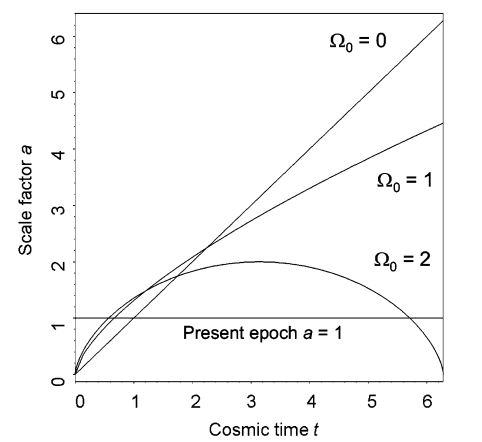
\includegraphics[width=0.65\textwidth]{grafica_scale_factor_timepp219Malcolm.png}
        \caption{}%\small{$\Omega = \varrho_0/\varrho_c$. Para  $\Omega_0 > 1$, el Universo colapsa a $a=0$. %Para $\Omega_0 <1$, el Universo se expande hasta el infinito y la velocidad de expansión es infinita como $a \rightarrow{\infty}$ . Por último, $\Omega_=1$. Para el del tiempo, este viene en términos del tiempo adimensional $H_0 t$. Siendo $t_0$ es el tiempo actual, cuando $\Omega_0 = 0$, $H_0 t_0=1$; $\Omega_0 = 1$, $ H_0 t_0 = 2/3$ y para $\Omega_0 = 2$, $H_0 t_0 = 0.57$. Las tres curvas tienen la misma pendiente $1$ para $a(1)$.}}
    \end{wrapfigure}
    
    
       En la figura 4 se muestran algunas soluciones a la ec. 7.21. Este gráfico ilustra la relación entre la dinámica y geometría de los modelos de Friedmann sin constante cosmológica. El eje $x$ viene en unidades de $H_0^{-1}$. Nótese la línea de la presente época $a=1$.  Las pendientes en ese punto son siempre $1$. Así mismo, la edad actual del Universo para cada parámetro es dada por la intersección de cada curva con la línea en $a=1$. 
    

    
    Este último caso, es un modelo de mundo vacío, o también se le conoce como {\textit{Modelo de Milne}} donde $a(t) = H_0 t$ y $\kappa = - (H_0/c)^2$. 
    
    
    \newpage
    
    Milne creía que la noción de que la gravedad deforma el espacio es creíble pero consideraba que esto no daba explicación acerca de su naturaleza. Que la materia y la gravedad estén enlazadas partiendo de la teoría de la Relatividad era algo de lo que dudó. Así, él construyó sus propia teoría coonocida como {\textit{relatividad cinemática}}, donde la gravedad no es un elemento principal. Basado en el principio cosmológico y la relatividad especial Milne crea una visión que explica la naturaleza de la gravedad y otras leyes físicas. 
    Su Universo consiste de una nube esférica de partículas (galaxias) las cuales se expenden dentro de un espacio plano, que es infinito y por lo tanto vacío. Bajo ideas de la relatividad especial, la expansión del Universo inicia en un punto del espacio: las partículas colisionan en todas las direcciones con velocidades que van desde cero hasta velocidades muy cercanas a la de la luz. También, el borde del Universo se expande a velocidades cercanas a las de la luz. Alrededor de cada una de las partículas, la distribución y velocidades de recesión de las otras partículas es isotrópica en el marco de referencia de esa partícula. En este Universo, la mayoría de las partículas se hallan agrupadas en los bordes de la nube (ver figura 5). Refiriéndose a esta idea como la relatividad cinemática, las partículas se mueven libremente sin ser afectadas por ninguna fuerza de modo que cada partícula tiene un comportamiento que simula el efecto de la gravedad. 
    Ya que hay un número infinito de galaxias, o partículas, este Universo tiene una masa también infinita. Su Univers finito y con borde, a través de cambios en los intervalos de espacio y tiempo, puede ser transformado en un Universo infinito y sin límites, el cual obedece la métrica de Robertson – Walker, ec. (21), y donde se expande el espacio, es homogéneo, isotrópico y con curvatura negativa, gemetría global hiperbólica, y está uniformemente poblado de galaxias. Esto es así ya que todas las galaxias que participan en la expansión no están desaceleradas y cualquiera en particular tiene la misma velocidad con respecto a un mismo observador fundamental. También, los tiempos cósmicos medidos en diferentes marcos de referencia están relacionados por las transformación de Lorentz estándar $t’ = \gamma(t – rv/c^2)$, siendo $\gamma = (1-v^2/c^2)^{-1/2}$. Las condiciones de isotropía y homogeneidad se aplican en el tiempo cósmico constante $t’$ en los marcos de referencia de todos los observadores fundamentales. 
    
    \newpage


   \begin{wrapfigure}[10]{r}{0.5\linewidth}                  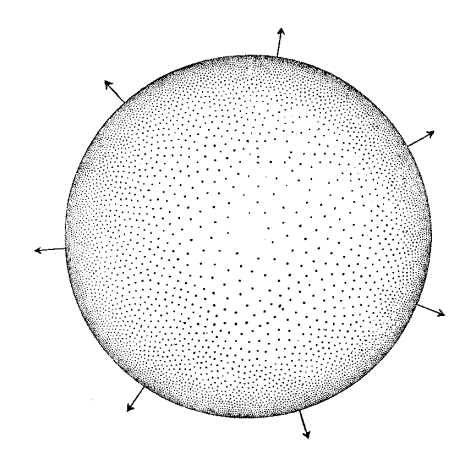
\includegraphics[width=0.65\textwidth]{milne_model.png}
        \caption{\footnotesize{El universo acotado de Milne se expande en el espacio.}}
    \end{wrapfigure}

 
Estas transformaciones de espacio y tiempo hace que las galaxias sean estacionarias en un espacio en expansión, y el Big Bang ya no existe como un punto en el espacio. Visto desde el punto de vista de la relatividad general, con la constante cosmológica cero y ya que Milne prescinde de la gravedad, entonces $G =0$, 

         \vspace{5cm}


    Las soluciones de (4.9) pueden ser escritas como: 
    
 

    
   \begin{itemize}

     \item $\Omega > 1$: 

        \begin{align}
            a & =A (1 - \cos \theta) \hspace{0.4cm} & t  = B(\theta - \sin \theta), \\
             A & = \frac{\Omega_0}{2(\Omega_0 -1 )} \hspace{0.4cm} & B  = \frac{\Omega_0}{2H_0( \Omega_0 - 1)^{3/2}}
        \end{align}
        
    \item $\Omega_0 <1$:

        \begin{align}
	        a & =A (\cosh \phi - 1) \hspace{0.4cm} &t = B(\sinh \phi - \phi ), \\
	        A & = \frac{\Omega_0}{2(1 - \Omega_0 )} \hspace{0.4cm} & B= \frac{\Omega_0}{2H_0(1 - \Omega_0)^{3/2}}.
        \end{align}

    \end{itemize} 

    Al final, todos los modelos van a tender a la dinámica del modelo crítico 
    
    
\subsection{Modelos de Friedmann con Constante Cosmológica}

    Einstein asumía que la estructura a gran escala del Universo era estática, entonces introdujo, de manera más bien [\textit{ad hoc}} la constante cosmológica para reconciliar esta visión con su teoría de la relatividad general pero nunca imaginó la importancia de su controversial constante cosmológica. $\Lambda$ aparecía en sus ecuaciones de campos como una constante. McVittie (1956) y otros, consideraban que $\Lambda$ era una constante de integración. McVittie enfatiza que, como una constancia de integración, $\Lambda$ no puede tener cualquier valor (McVittie, 1959, p. 35) (McVittie, G. C., 1956, General Relativity and Cosmology (Chapman and Hall, London).)  Más tarde, en 1933, Lema\^itre sugiere que $\Lambda$ puede ser interpretada como una densidad de energía de vacío (Lema\^itre, 1933), interpretación bastante acertada con respecto a la cosmología moderna, conocida como la {\textit{energía oscura}}, un problema todavía no resuelto. 

    \subsubsection{Constante Cosmológica y la Densidad de Energía del Vacío}
    
    Recordando que las 3.4 y 3.5 
    
    \begin{empheq}[box=\fbox]{align}
        \ddot{a} = - \frac{4 \pi G}{3} a \left( \varrho + \frac{3p}{c^2} \right) + \frac{1}{3} \Lambda a, \\
         \notag \\ 
        \dot{a}^2 =  \frac{8 \pi G \varrho}{3} a^2 - \frac{c^2}{R'^2} + \frac{1}{3} \Lambda a^2, 
    \end{empheq}
    
    son las ecuaciones de campo de Einstein que incluyen la $\Lambda$. Para Universos llenos de polvo, $3p/c^2=0$, por lo que ahora 3.4  se simplifica a 
    
    
    \begin{equation}
         \ddot{a} = - \frac{4 \pi G a \varrho  }{3}+ \frac{1}{3} \Lambda a =- \frac{4 \pi G\varrho_0 }{3a^2}+ \frac{1}{3} \Lambda a. 
    \end{equation}
    
    La expresión 4.14 nos dice que, así se considere un Universo vacío donde $\varrho=0$, hay una fuerza neta que actúa sobre una partícula de prueba. Para el caso en que $\Lambda$ sea positiva, puede ser interpretada como una especie de ``fuerza repulsiva'', asumida opuesta a la gravedad, de un vacío (Zeldovich, 1968) Desde el punto de vista de la física clásica no existe una explicación obvia para este término. 
    
    Desde el punto de vista de la teoría cuántica de campos, se introdujo el campo de Higgs en la teoría de interacciones débiles del modelo estándar para eliminar singularidades en la teoría y para dotar de masa a los bosones $W^{\pm}$ y $Z^0$,  (Zeldovich, 1986).  Zeldovich establece que los campos de Higgs tienen la propiedad de ser campos escalares, donde las ecuaciones de estado tienen presiones negativas $p=- \varrho c^2$, y que son diferentes de los campos vectoriales del electromagnetismo o los campos tensoriales de relatividad general. 
    
    El tensor energía - momento de un vacío tiene una ecuación de estado de presión negativa $p=- \varrho c^2$, donde $p$ puede ser interpretada como una ``tensión'' más que una presión. Cuando el vacío se expande, el trabajo hecho $p dV$  al expandirse de $V$ a $V + dV$ es $- \varrho c^2 dV$ de modo que, durante la expansión, la densidad de masa - energía del campo de presión negativa permanece constante. Este resultado puede ser igualmente obtenido si se cosidera $\varrho$ constante en (3.23). 
    
    Desde el punto de vista de la teoría cuántica de campos, se puede hacer un análisis para estimar la densidad de energía de los campos vacíos. La energía de punto cero de campos constribuye con la densidad de la energía oscura. La suma sobre las energías de modo de punto cero debe ser limitada a una frecuencia alta (o distancia corta) hasta la cual el modelo físico tenga sentido. Así, la integral de la energía de punto cero ($k/2$) de modos normales (de número de onda $k$) de un campo escalar bosónico sin masa ($\Phi$) hasta un número de onda máximo $k_{max}$ en la que la teoría se rompe, da la densidad de energía del vacío 
    
  \begin{equation}
       \varrho_{vac} = \int_0^{k_{max}}{\frac{4\pi k^2 dk }{(2\pi)^3} \frac{k}{2}}.
  \end{equation}
  
  Tomando el límite
    
   \begin{equation}
       \varrho_{vac} = \lim_{L \to \infty}{\frac{E_0}{L^3}} = \hbar \frac{k^4_{max}}{16 \pi^2}.
   \end{equation}
    
    
    Carroll, Press y Turner (Carroll, et al., 1992), en su enfoque, toman la energía a la cual teoría de campos se rompe debido a efectos gravitatorios cuánticos que toman lugar en la escala de energía de Planck $E*\sqrt{\hbar c^5/G}  \approx 10^{19} \mathrm{GeV}$, de manera que si
    $$k_{max} = \frac{E*}{\hbar},$$
    
    \begin{equation}
        \varrho_{vac} \approx 10^{95} \mathrm{kg m^{-3}}.
    \end{equation}
    
    
    Desde un punto de vista similar, Peacock (Peacock, 2000) , consierando el Principio de Incertidumbre de Heisenberg, el cual estable que una par de partículas virtuales de masa $m$ pueden existir para un tiempo $t \sim \hbar mc^2$ que corresponde a una separación máxima de $x \sim \hbar/mc$. De esta manera, la densidad típica de campos de vacío 

    \begin{equation}
	    \varrho \sim \frac{m}{x^3} \approx \frac{c^3m^4}{\hbar^3}.
    \end{equation}
    
    Debido a que la densidad de masa en campos vacíos es invariable con el tiempo cósmico, entonces adoptando la masa de Planck $m = m_P = \sqrt{hc/G} = 5.4 \times 10^{-8} \, \mathrm{kg} = 3 \times 10^{19} \, \mathrm{GeV}$, la densidad de masa obtenida es

    \begin{equation}
        \varrho_{vac} = \sim 10^{97} \, \mathrm{kg m^{-3}}
    \end{equation} 
    
    Actualmente, hay evidencia convincente de que $\Lambda$ tiene un valor finito con una densidad de masa 
    \begin{equation}
        \varrho_v \approx 6 \times 10^{-27} \mathrm{kg \, m^{-3}},
    \end{equation} 

    alrededor de unas $10^{120}$ veces menos que el valor predicho, diferencia que genera un gran problema en la física. El detalle acá es explicar cómo puede este valor variar tan bruscamente. 
    
    Con el desarrollo de la idea del rompimiento de simetría en el modelo estándar de partículas, se planteó una relación de la expansión y enfriamiento del Universo con una secuencia de transiciones de fase que acompañan al rompimiento de simetría. Cada transición de fase de primer orden tiene un calor que parece como una contribución a una constante cosmológica dependiente del tiempo $\Lambda(t)$ o densidad de energía oscura. La disminución del valor de esta densidad de energía oscura en cada transición de fase es mayor que un valor presente. Una posible respuesta es que la energía oscura ahora es despreciada, lo cual parece descabellado pero condujo al escenario de la inflación que tomó lugar en el Universo muy temprano ($\sim 10^{-36} - 10^{-33} s$). Desde esta visión, este es exactamente el tipo de campo que condujo la expansión inflacionaria. Se debe encontrar una explicación al hecho de que $\varrho_v$ decrece por un factor $10^{120}$ al final de la era inflacionaria. U valor de $10^{-120}$ es un valor tan pequeño que, como se mencionó arriba, podría considerarse que $\Lambda=0$ en el modelo de Friedmann. 

   Es posible asociar la ``repulsión del vacío' de Zeldovich con una densidad de masa $\varrho_v$ y con la densidad de energía del vacío o la energía oscura en la presente época. Consideremos entonces un parámetro de densidad relacionada con la energía oscura $\Omega_{\Lambda}$. Reescribimos 4.16 como:
   
   \begin{align}
         \ddot{a} & = - \frac{4 \pi Ga}{3}  \left( \varrho + \frac{3p}{c^2} \right) + \frac{1}{3} \Lambda a, \\
          \ddot{a} & = - \frac{4 \pi Ga}{3}  \left( \varrho_m + \varrho_v + \frac{3p_v}{c^2} \right),
   \end{align}
       
    donde estamos considerando la densidad de `polvo'$\varrho_{m}$, y consideramos la densidad del vacío $\varrho_v$ y la presión $p_v$. Siendo ahora $p_v = - \varrho_vc^2$, se sigue
    
    \begin{equation}
        \ddot{a} = - \frac{4 \pi G a}{3}  \left( \varrho_m -2\varrho_v \right).
    \end{equation}
    
    En este caso, $\varrho_m = \varrho_0/a^3$, mientras $\varrho_v = cte$.Y sustituyendo
    
    \begin{equation}
         \ddot{a} = - \frac{4 \pi G \varrho_0}{3 a^2} + \frac{8 \pi G \varrho_v a}{3}.
    \end{equation}
    
    Haciendo una revisión a la relación 4.16,
    
    \begin{equation*}
         \ddot{a} = - \frac{4 \pi G a \varrho  }{3}+ \frac{1}{3} \Lambda a =- \frac{4 \pi G\varrho_0 }{3a^2}+ \frac{1}{3} \Lambda a. 
    \end{equation*}
    
    la cual tiene la misma forma de 4.26, se puede identificar el término $\Lambda$
    
    \begin{equation}
        \Lambda = 8\pi G\varrho_v.
    \end{equation}
    
    Si nos referimos a la época actual, $a=1$, se tiene 
    
    
    \begin{equation}
         \ddot{a} = - \frac{4 \pi G \varrho_0}{3} + \frac{8 \pi G \varrho_v }{3}.
    \end{equation}
    
    De la misma manera que se determinó $\Omega_0$ (ec. 4.4), nosotros podemos asociar un parámetro a la densidad del vacío y la constante cosmológica. Así:
    
    \begin{equation}
         \Omega_{\Lambda} = \frac{\varrho_v}{\varrho_c} = \frac{8 \pi G \varrho_v}{3 H_0^2}.
     \end{equation}
    
    De manera que, sustituyendo el término $\varrho_v$ en 4.27, 
    
    \begin{equation}
        \Lambda = 3 H_0^2 \Omega_{\Lambda}.
    \end{equation}
    
    Y así podemos repetir toda la deducción anterior hecha para el caso sin costante cosmológica. Sustituyendo en las ecuaciones de movimiento, 4.16 y 4.17 el valor de $\Lambda$ y $\varrho_0$,
    
   
       \begin{empheq}[box=\fbox]{align}
            \ddot{a} & = - \frac{\Omega_0 H_0^2 }{ 2a^2} +  H_0^2 \Omega_{\Lambda} a, \\
            \notag \\
            \dot{a}^2 & = \frac{\Omega_0 H_0^2  }{a} - \frac{c^2}{R'^2} + H_0^2 \Omega_{\Lambda} a^2.
        \end{empheq}
         
    A continuación, se sustityen los valores de $a$ y $\dot{a}$ en 4.34 para la época actual, obteniéndose
    
    \begin{align}
        H_0^2 & = \Omega_0 H_0^2  - \frac{c^2}{R'^2} +  H_0^2 \Omega_{\Lambda}, \notag \\
        \frac{c^2}{R'^2} & = H_0^2 [(\Omega_0 + \Omega_{\Lambda}) - 1] \hspace{1cm} \text{o} \\
        \notag \\
        \kappa & = \frac{1}{R'^2} = \frac{[(\Omega_0 + \Omega_{\Lambda})]}{c^2/H_0^2}.
    \end{align}
        
   De aquí, la condición de que las secciones espaciales son espacios planos Euclideos se escribe 
   
   \begin{equation}
      (\Omega_0 + \Omega_{\Lambda}) = 1. 
   \end{equation}
  
   
   Recordando que el radio de curvatura, $R_c$, cambia con el factor de escala, $R_c=aR'$, si la curvatura del espacio es cero en este momento, también debió serlo en todos los tiempos del pasado. 
    
    
    %%\subsection{Variando la Ecuación de Estado de la Energía del Vacío }
    
    \subsection{Consideraciones Generales de la Dinámica de Modelos de Mundo con $\Lambda \neq 0$. }
    
    La importancia de estos modelos es que ayudan a determinar y mejoras valores de los parámetros cosmológicos. Algunas consideraciones son: 
    
    \begin{itemize}
        \item $\Lambda < 0$: 
        
            En estos modelos existe una fuerza adicional a la gravedad la cual ralentiza la expansión del Universo. Si revisamos la relación (4.18), podemos extraer que independientemente de cuán pequeños sean los valores de $\Omega_{\Lambda}$ y  $\Omega_{0}$ , la expansión del Universo se va a revertir. 
        
        \item $\Lambda, \Omega_{\Lambda} > 0$:
        
            Los modelos con constante cosmológica positiva conduce a una ``fuerza repulsiva'', contraria a la fuerza de la gravedad. Son modelos mucho más interesantes los cuales tienen una tasa de expansión mínima. Si $\ddot{a} = 0$ en ec. (4.33), obtenemos el factor de escala mínimo, $a_{min}$ e insertando este valor en (4.34), podemos conocer la tasa mínima de expansión, $\dot{a}_{min}$. Así:
            
            
        \begin{empheq}[box=\fbox]{align}
            a_{min} & = \left( \frac{\Omega_0}{ 2\Omega_{\Lambda}} \right)^{1/3}, \\
            \notag \\
            \dot{a}_{min}^2 & = \frac{3 H_0^2 }{2} (2\Omega_{\Lambda} \Omega_0^2 )^{1/3} - \frac{c^2}{R'^2}.
        \end{empheq}
        
        
    \end{itemize}

\vspace{2cm}
    
     Analicemos la ec. (4.38). 
     
     \begin{itemize}
         \item Cuando el lado derecho de la igualdad es mayor que cero, su comportamiento es reflejado en la fig. 6a. Para valores grandes de $a$, la dinámica sigue  a la  de Universos de Sitter
         
        \begin{equation}
        a(t) \propto \exp \left[\left(\frac{\Lambda}{3} \right)^{1/2} t \right] = \exp (\Omega^{1/2}_{\Lambda} H_ot)
        \end{equation}
    
        \item De la misma manera, si el lado derecho de 4.38 es menor que cero, de la figura 6b, la función $a(t)$ tiene dos ramas. Existe un rango de factores de escala para los cuales no hay solución.
        
            \begin{itemize}
                \item [Rama A:] La dinámica está dominada por la constante $\Lambda$; la fuerza repulsiva es tan fuerte que el Universo nunca se contrajo a una escala a la que la fuerza atractiva de la gravedad pudiera contrarestar o vencer su efecto. 
        
                \item [Rama B:] En este caso, el Universo nunca se expandió alcanzando valores suficientemente grades del factor de escala $a$ como para que la fuerza repulsiva transportada a través de $\Lambda$ pudiera evitar el colapso del Universo. No presenta una singularidad inicial, por lo que el Universo ``rebotó''  bajo la influencia de la fuerza repulsiva. 
            \end{itemize}
            
            En el caso límite, en el que el parámetro de densidad $\Omega_0 = 0$ la dinámica del modelo y su solución vienen dadas por
            
            \begin{align}
                \dot{a}^2 & = H_0^2 [\Omega_{\Lambda} a^2 - (\Omega_{\Lambda}-1)], \\
                a & = \left(\frac{\Omega_{\Lambda} - 1}{\Omega_{\Lambda}} \right)^{1/2} \cosh \Omega_{\Lambda}^{1/2} H_0 \tau.
            \end{align}
            
            De esta última relación, $\tau = t - t_{min}$, el cual es medido desde el momento en el que el Universo `rebotó', i.e., cuando $a= a_{min}$. El comportamiento asintótico que presenta es debido al colapso exponencial que experimenta y son soluciones exponenciales de Sitter
            
            \begin{equation}
                a = \left(\frac{\Omega_{\Lambda} - 1}{\Omega_{\Lambda}} \right)^{1/2} \exp (\pm \Omega_{\Lambda}^{1/2} H_0 \tau).
            \end{equation}
            
            En estos Universos `rebotantes', el valor más pequeño de $a$, $a_{min}$, es aquel con el desplazamieto al rojo más grade que un objeto pueda tener. 
       
       \item En tercer lugar, tenemos el caso en el que $\dot{a_{min}} \approx 0$. La figura 6c ilustra lo que se conoce como el {\textit{modelo de Eddington - Lema\^itre}} donde $\dot{a_{min}} = 0$. La interpretación de A, B y C es:
       
       \begin{itemize}
           \item[A:] El Universo se expandió desde un punto en el origen en algún tiempo pasado finito y eventualmente alcanzará un estado estacionario en el futuro infinito. 
           \item[B:] El Universo se está expandiendo lejos de una solución estacionaria en el pasado infinito. 
           \item[C:] Es un estado estacionario y además inestable ya que, de ser perturbado, el Universo va a moverse hacia el estado que colapsa A, o hacia B. 
           
           Para el caso del Universo estático de Einstein, el estado estacionario sería alcanzado en el presente día. Para estos modelos con $\dot{a} = 0$, el valor de la constante cosmologica puede ser obtenido de la ec. (4.37):
           
           \begin{align}
               \Lambda & = \frac{3}{2} \Omega_0 H_0^2 (1 + z_c)^3 \hspace{0.4cm} \text{o equivalentemente} \\
               \Omega_{\Lambda} & = \frac{\Omega_0}{2} (1 + z_c)^3,
           \end{align}
           
           siendo $z_c$ el desplazamiento al rojo de objetos estacionarios. 
       \end{itemize}
       
       
    \end{itemize}
    
    
    
     \begin{figure}[H]         
     \centering
     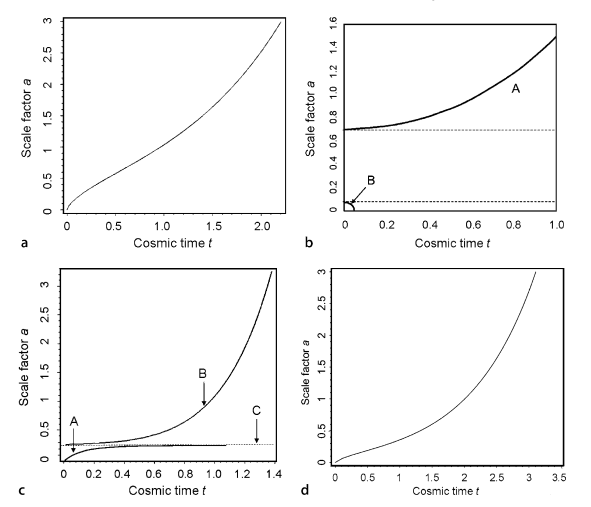
\includegraphics[width=1.0\textwidth]{graficos73_pp226Mlalcon.png}
        \caption{\footnotesize{Modelos con $\Lambda \neq 0$ }. En el gráfico {\bf{a}} los parámetros cosmológicos son $\Omega_0=0.3$ y $\Omega_{\Lambda}= 0.7$, los cuales son valores que se ajustan bastante bien a las estimaciones actuales. {\bf{b}} ilustra el Universo `rebotante'con $\Omega_0 = 0.05$ y $\Omega_{\Lambda}=5$. El cero en el tiempo cósmico se ha establecido para cuando $\dot{a}=0$. {\bf{c}} muestra un modelo de Eddington - Lema\^itre que tiene un corrimiento al rojo estacionario $z_c = 3$, lo que es equivalente a un factor de escala $a=0.25$. El modelo {\bf{d}} tiene parámetros $\Omega_0 = 0.01$ y $\Omega_{\Lambda}= 0.99$, donde la edad del Universo puede exceder por mucho a $H_0^{-1}$. Por último, {\bf{a}} y {\bf{d}} son conocidos como los modelos de Lema\^itre. (Bondi, 1960)}
     \end{figure}
    
    
    Ya que los Universos estáticos de Eddington - Lema\^itre no presentan dinámica $\dot{a}=0$, podemos usar (4.44) y sustituirlo en (4.34) para obtener
    
    \begin{equation}
        \Omega_0 = \frac{2}{ (1 + z_c)^3 - 3  (1 + z_c) + 2} = \frac{2}{ z_c^2(z_c + 3)},
    \end{equation}
    
    lo que muestra una relación uno a uno entre la densidad media de materia en el Universo $\Omega_0$ y el desplazamiento al rojo en el estado estacionario $z_c$.
    
    La figura 7 ilustra los modelos de mundo con $\Lambda \neq 0$  resumidos en un plot de $\Omega_0$  vs. $\Omega_0 + \Omega_{\Lambda}$ (Carroll et a., 1992). 
    
    \begin{itemize}
        \item Los modelos con $\Lambda=0$: encontrados a lo largo de una línea de $45^{\circ}$ y que parten de cero en ambos ejes. 
    \end{itemize}
    
    De la ec. (4.36) puede visualizarse que la geometría de los modelos depende del valor que tenga $\Omega_0 +  \Omega_{\Lambda}$. La unidad separa las geometrías abiertas de los cerradas. 
    
    Los modelos que tuvieron un pasado singular y esos que `rebotaron' son separados por la línea correspondiente a modelos que fueron estacionarios en el pasado, y vienen dadas por las ecs. (4.43) o (4.44), y (4.45). También se indican los valores de los desplazamientos al rojo estacionarios en la parte inferior derecha del diagrama, donde encontramos los modelos `merodeadores' ({\textit{loitering}}) (llamados así por Carroll et al.). La línea divisoria también separa aquellos Universos que se expandirán infinitamente de aquellos que volverán a colapsar en un 'Gran Crujido' ({\textit{Big Crunch}}) en el futuro. Por ejemplo, usando (4.45) se encuentra que el modelo que es estacionario a un factor de escala $a=1.5$ o $(1+z_z)=2/3$, tiene un $\Omega_0=1.69$. Así, de (4.44) $\Omega_{\Lambda} =0.25$, de esta manera $\Omega_{\Lambda} + \Omega_0 = 1.94$, puntos que se encuentran en la línea que separa a los modelos que se expandirán infinitamente de esos que colapsarán en un tiempo finito. 
    
    
    \begin{itemize}
        \item Los modelos con constante cosmológica positiva pueden tener edades mayores a $H_0^{-1}$. En casos límites como los modelos de Eddington - Lema\^itre con $\dot{a}_{min}=0$ en el pasado infinito, el 
        
       Los conocidos {\textit{modelos de Lema\^itre}} son otro posible caso de Universos con edades mayores a $H_0^{-1}$, donde el valor de $\Omega_{\Lambda}$ es tal que $\dot{a}_{min} >0$. Como s mencionó arriba, un ejemplo de estos modelos es el de la figura 6d. 
    \end{itemize}
    
    
    \begin{figure}[H]         
     \centering
     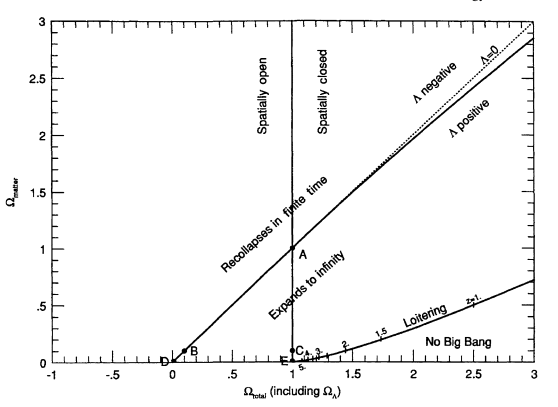
\includegraphics[width=1.0\textwidth]{friedmann_worldspp228_Malcolm.png}
        \caption{\footnotesize{Clasificación de los modelos de Friedmann con $\Omega_{\Lambda} \neq 0$, son ilustradosdos en un gráfico de $\Omega_0$ vs. $\Omega_{\Lambda} + \Omega_0$ (Carroll et al., 1992). Los modelos de Eddington - Lema\^itre son aquellos a lo largo de la línea etiquetada como {\textit{loitering} }.}}
     \end{figure}
    
    Existe una fuerte evidencia de que Universos con geometría plana tiene un valor de $\Omega_{\Lambda} + \Omega_0$ cercano a la unidad. La dinámica de estos modelos planos con diferentes valores de $\Omega_0$ y $\Omega_{\Lambda}$ se muestran en la figura 8. Dichos modelos ilustran cómo la edad del Universo puede ser más grande que $H_0^{-1}$ para valores de $\Omega_{\Lambda}$ suficientemente grandes. 
    
    
    \begin{figure}[H]         
     \centering
     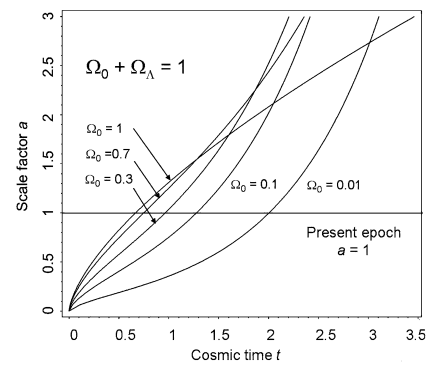
\includegraphics[width=0.9\textwidth]{flat_models_pp229_Malcolm.png}
        \caption{\footnotesize{Dinámica de modelos con geometría plana, $\Omega_{\Lambda} + \Omega_0 = 1$. El eje $x$ tiene unidades de  $H_0^{-1}$. Este gráfico puede ser comparado con la figura 4, el cual representa el caso donde $\Omega_{\Lambda}=0$ .}}
     \end{figure}
    
    \subsection{Cosmología Observacional}
    
    La cosmología actual es dominada por modelos de mundo con un valor finito de la constante cosmológica, sin embargo, modelos con $\Omega_{\Lambda}$ son igualmente considerados para hacer comparaciones y así obtener mejores estimaciones sobre parámetros cosmológicos.
    
    \subsubsection{Parámetro de Descaleración}
    
    De secciones anteriores, la constante de Hubble $H_0$ ha sido introducida, y sabemos que mide la tasa de expansión del Universo en el tiempo actual, i.e., $a=1$. Así mismo, también podemos considerar el {\textit{parámetro de desaceleración}} $q_0$ el cual es adimensional y en la presente época viene definido como
    
    \begin{equation}
        q_0= - \left( \frac{a\ddot{a}}{\dot{a}^2}\right)_{t_0}.
    \end{equation}
    
    Haciendo las consideraciones de $a(t_0)=1$ y $\dot{a}=H_0$ para la presente época, 4.46 se convierte en: 
    
    \begin{equation}
        q_0= - \frac{\ddot{a}}{H_0^2}.
    \end{equation}
    
    
    Haciendo uso de la ecuación Dinámica (), y sustituyendo en 4. se obtiene

\begin{equation}
	q_0 = \frac{\Omega_0}{2} - \Omega_{\Lambda}.
\end{equation}

Usando los valores preferenciales de $\Omega_{\Lambda} = 0.7$ y $\Omega_0 = 0.3$, nosotros obtenemos un valor del parámetro de desaceleración $q_0 = -0.55$, lo cual indica que efectivamente, el Universo se está desacelerando en la presente época producto de que la energía oscura domina sobre la gravedad. 

Algunos resultados siguen acerca del desplazamiento al rojo y la relación que guarda con el tiempo cósmico, medidas de distancias, diámetro angular, densidad de flujo y volumen comóvil, para modelos de mundo con y sin el término de constante cosmológica $\Omega_{\Lambda}$. En lo que sigue, un análisis matemático es realizado para cada una de las relaciones. 

\subsubsection{Relación Tiempo Cósmico – Corrimiento al Rojo}

Para la relación del dezplazamiento al rojo con el tiempo cósmico, podemos combinar las ecs. 4.33 y 4.34. Así, 

    \begin{align}
	    \dot{a}^2 &= \frac{\Omega_0 H_0}{a} – H_0^2 [(\Omega_0 + \Omega_{\Lambda} -1] +  \Omega_{\Lambda}H_0^2 a^2, \notag \\
	    \dot{a} & = H_0 \left[ \Omega_0 \left( \frac{1}{a} - 1 \right) + \Omega_{\Lambda}(a^2 - 1) + 1 \right]^{1/2},
    \end{align}

y considerando que $a = (1+z)^{-1}$,

    \begin{equation}
	    \frac{dz}{dt} = - H_0(1+z) [ (1+z)^2 (\Omega_0 z + 1) - \Omega_{\Lambda} z (z+2) ]^{1/2}.
    \end{equation}

    El tiempo cósmico, desde el Big Bang hasta cualquier $z$ puede ser medido por integrar 7.46, con límites desde $z = \infty$ hasta $z$. 

    \begin{equation}
	    t = \int_0^t{dt} = - \frac{1}{H_0} \int_{\infty}^z{\frac{dz}{  (1+z)[(1+z)^2 (\Omega_0 z + 1) - \Omega_{\Lambda} z (z+2) ]^{1/2}}.} 
	\end{equation}


    Obtenida la relación anterior, se tiene:

        \begin{itemize}
	        \item Modelos con $\Omega_{\Lambda}=0$. 

		Para un parámetro de densidad $\Omega_0 >1$ es posible escribir 

		$$ 
		x = \frac{(\Omega_0-1)a}{\Omega_0} = \frac{(\Omega_0-1)}{\Omega_0 (1+z)} , 		
		$$
		
		obteniendo así que la relación corrimiento al rojo -  tiempo cósmico 

		\begin{equation}
			t(z) = \frac{\Omega_0}{H_0( \Omega_0 - 1)^{3/2}}[\sin^{-1} x^{1/2} - x^{1/2} (1-x)^{1/2}].
		\end{equation}
		
		Y haciendo el mismo procedimiento pero para el caso en el que $\Omega_0 < 1$,

	    $$
	    y = \frac{(1- \Omega_0)a}{\Omega_0} = \frac{(1-\Omega_0)}{\Omega_0 (1+z)},
	    $$

    encontrándose

    \begin{equation}
	    t(z) = \frac{\Omega_0}{H_0(1 - \Omega_0)^{3/2}}[ y^{1/2} (1+y)^{1/2} + \sinh^{-1} y^{1/2}].
    \end{equation}
    
    Y si asumimos corrimientos al rojo muy altos, $z>>1$ y $\Omega_0 z >>1$, entonces 4.52 y 4.53 se reducen a 

    \begin{equation}
        t(z) = \frac{2}{3H_0 \Omega_0^{1/2}} z^{-3/2},
    \end{equation}
		
		
		y entonces hallar la edad del Universo para diferentes valores de $\Omega_0$ es posible. 

        \begin{itemize}

            \item[-] Para $\Omega_0>1$:

            \begin{equation}
	           t_0 = \frac{\Omega_0}{H_0(\Omega_0 - 1)^{3/2}} \left[ \sin^{-1} \left( \frac{ \Omega_0 - 1}{\Omega_0} \right)^{1/2} - \frac{{(\Omega_0 - 1)}^{1/2}}{\Omega_0 } \right].
            \end{equation}
            
            \item[-] $\Omega_0=1$:
            
            \begin{equation}
                t_0 = \frac{2}{3H_0}.
            \end{equation}

        \item[-] $\Omega_0<1$:
        
        \begin{equation}
       t_0 = \frac{\Omega_0}{H_0(1-\Omega_0)^{3/2}} \left[   \frac{(   1- \Omega_0)^{1/2}}{\Omega_0}  - \sinh^{-1} \left( \frac{{ 1-\Omega_0}}{\Omega_0 } \right)^{1/2} \right].
            \end{equation}
            
        \end{itemize}
        
        
        Los casos más útiles y simples son aquellos con $\Omega=1$, ec. (4.56); el caso de un Universo vacío tipo Milne, $\Omega_0 =0$ y la edad es $H_0^{-1}$; y el caso con $\Omega_0=2$, cuya edad calculada es $0.571 H_0^{-1}$. 
        
        \item Modelo con $\Omega_{\Lambda} \neq 0$:
        
        Regresando a (4.52), podemos encontrar la relación del desplazamiento al rojo con el tiempo cósmico para una valor finito de $\Omega_{\Lambda}$. Los modelos con curvatura del espacio cero son de particular interés y para que esto ocurra, de (4.36) que $R'\rightarrow{\infty}$, cumpliéndose la condición (4.37) $(\Omega_{\Lambda}  + \Omega_0) =1$ para espacios planos Euclideos. (4.52) se reduce a:
        
        \begin{equation}
             t = \int_0^t{dt} = - \frac{1}{H_0}\int_{\infty}^z{\frac{dz}{(1+z)[\Omega_0(1+z)^3+\Omega_{\Lambda}]^{1/2}}},
        \end{equation}
        
        con solución 
        
        \begin{align}
            t &= \frac{2}{3H_0\Omega_{\Lambda}^{1/2}} \ln \left(\frac{1+\cos \theta }{\sin \theta} \right)   \hspace{0.5cm} \text{donde:} \notag \\
            \tan \theta &= \left(\frac{\Omega_0}{\Omega_{\Lambda}} \right)^{1/2} (1+z)^{3/2}
        \end{align}
        
        Para la época presente, $z=0$. Así: 
        
        \begin{equation}
            t_0 = \frac{2}{3H_0\Omega_{\Lambda}^{1/2}} \ln \left[\frac{1 + \Omega_{\Lambda}^{1/2}}{(1-\Omega_{\Lambda})^{1/2}} \right].
        \end{equation}
        
        De esta última relación, es posible encontrar modelos de Friedmann que tengan edades mayores que $H_0^{-1}$ y que además, sean espacios planos. Para valores del los parámetros $\Omega_0 = 0.1$ y $\Omega_{\Lambda}=0.9$, la edad del Universo es de $1.28 H_0^{-1}$; para valores ideales de $\Omega_{\Lambda} = 0.7$ y $\Omega_0=0.3$, se tiene un Universo con $0.964 H_0^{-1}$. 
    
    \end{itemize}
    
    \subsubsection{Medidas de Distancias en función del Desplazamiento al Rojo}
    
   Nos interesa ahora obtener valores de la coordenada de distancia comóvil, $r$ y la medida de la distancia $D$, para esto vamos a recordar la relación (2.3)
   
   \begin{equation}
       dr = - \frac{cdt}{a(t)} = -c \, dt (1+z).
   \end{equation}
    
    Nuevamente, de (4.51)
    
    \begin{equation}
         dr = - \frac{cdt}{a(t)} = \frac{c}{H_0}  \frac{dz}{[ (1+z)^2 (\Omega_0 z + 1) - \Omega_{\Lambda} z (z+2) ]^{1/2}},
    \end{equation}
    
    e integrando desde $z=0$ a $z=0$
    
    \begin{equation}
        r = \frac{c}{H_0} \int_0^z{\frac{dz}{[ (1+z)^2 (\Omega_0 z + 1) - \Omega_{\Lambda} z (z+2) ]^{1/2}}}.
    \end{equation}
    
    
    Note que determinar $D$ está implícito ya que $D = R' \sin(r/R')$, donde $R'$ es la hallada en la ec. (4.35), $ c^2/R'^2  = H_0^2 [(\Omega_0 + \Omega_{\Lambda}) - 1]$. 
    
    A continuación, repetimos el mismo análisis de modelos con $\Omega_{\Lambda} =0$ y $\Omega_{\Lambda} \neq 0$. 
    
    
    \begin{itemize}
	        \item Modelos con $\Omega_{\Lambda=0}$. 

		Considerando $\Omega_0 >1$, la última expresión se reduce a 
		
		\begin{align}
		    r &= \frac{c}{H_0} \int_0^z{\frac{dz}{1+z) (\Omega_0 z + 1)^{1/2}}}, \\
		    r& =  \frac{2c}{H_0 (\Omega_0 z -1)} \left[ \tan^{-1} \left(\frac{\Omega_0 z + 1}{\Omega_0 z -1} \right)^{1/2} - \tan^{-1} (\Omega_0 -1)^{-1/2} \right].
		\end{align}
     
     Y, en el caso en que el parámetro de densidad $\Omega_0 <1$, se tiene
     
     \begin{equation}
         D = \frac{2c}{H_0 \Omega_0^2( 1+z)} \{ \Omega_0 z+ (\Omega_0 - 2) [(\Omega_0 z+1)^{1/2} - 1 ] \}.
     \end{equation}
    
    La expresión (4.67) es la famosa fórmula derivada por Mattig (Mattig, 1959), la cual es correcta para diferentes valores de $\Omega_0$. Por ejemplo, para $\Omega_0 = 0$, que es el Universo de Milne, la expresión se convierte en 
    
    
    \begin{equation}
         D = \frac{cz}{H_0} \frac{\left( 1 + \frac{Z}{2} \right)}{(1+z)}.
    \end{equation}
    
    Las figuras 9 y 10 muestran las variaciones de $r$ y $D$ con $z$ para un rango de $\Omega_0$. 
    
    \item Modelos con $\Omega_{\Lambda} \neq 0$:
    
    Por lo general, se puede evaluar $r$ y $D$ por integración numérica. Por ejemplo, modelos planos donde $(\Omega_{\Lambda} + \Omega_0)=1$ (ec. 4.37), para diferentes valores de $\Omega_0$ se muestran el la figura 11. Debido a la geometría de estos modelos planos, $R'=\infty, r = D$.
    
    
    
    \end{itemize}
    
    
    Un análisis más profundo podemos hacer de estas tres figuras. Primero, para el caso de las figuras 9 y 10 ($\Omega_{\Lambda} =0$), note cómo para un parámetro de densidad mayor, tanto la coordenada de distancia radial comóvil, $r$, así como la distancia medida, $D$, son más grandes para un cierto desplazamiento al rojo, $z$. Esto puede ser justificado por considerar el tiempo que viaja la luz a lo largo de la geodésica radial desde el objeto hasta el observador en la Tierra. Mientras el valor del parámetro de desacaleración universal, $q_0$, es menor (una aceleración mayor) mayor es la distancia que debe recorrer la luz para alcanzar la Tierra. Lo mismo ocurre para la figura 11, entre mayor sea el valor de $\Omega_{\Lambda}$ mayor será el tiempo de viaje de la luz hasta la Tierra. Así mismo, es importante observar la influencia de la geometría espacial curva en las figs. 9 y 10. Para el caso en que $\Omega_0 = 0$, las geometrías coinciden por ser planas en ambos casos. Ya para otros valores, la ubicación geométrica de las medidas de $D$ en figura 10 divergen en el modelo debido a las geometrías hiperbólicas $\Omega_0 <1$ y esféricas $\Omega_0 >1$. 
    
\begin{figure}[H]
        \begin{minipage}[b]{0.5\linewidth}
        \centering
        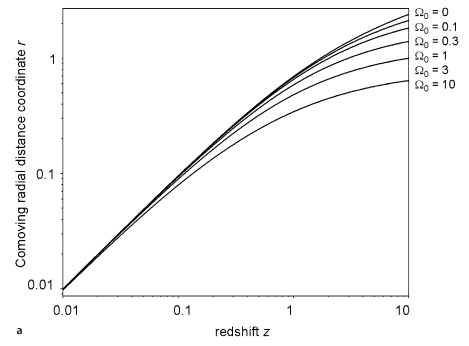
\includegraphics[scale=0.42]{redshift_r7a.png}
        \caption{\footnotesize{Variación del desplzamiento al rojo de la coordenada radial comóvil $r$ para $\Omega_{\Lambda}=0$.}}
        %\label{fig:figura1}
    \end{minipage}
        \hspace{0.5cm}
    \begin{minipage}[b]{0.4\linewidth}
        \centering
        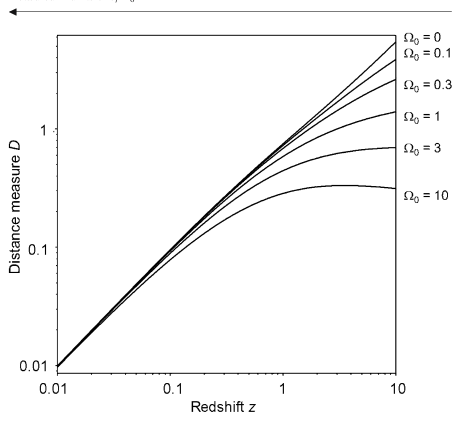
\includegraphics[scale=0.4]{redshift_r77.png}
        \caption{\footnotesize{Variación de $z$ de la distancia medida $D$ (en unidades de $c/H_0$) para $\Omega_{\Lambda}=0$. }}
        %\label{fig:figura2}
    \end{minipage}
\end{figure}


    
    \begin{figure}[H]         
     \centering
     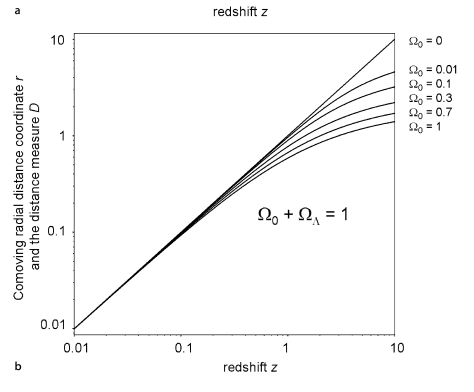
\includegraphics[width=0.7\textwidth]{redshift_r76b.png}
        \caption{\footnotesize{Dinámica de modelos con geometría plana, $\Omega_{\Lambda} + \Omega_0 = 1$. El eje $x$ tiene unidades de  $H_0^{-1}$. Este gráfico puede ser comparado con la figura 4, el cual representa el caso donde $\Omega_{\Lambda}=0$ .}}
     \end{figure}
    
    \subsubsection{Relación del Diámetro Angular con el Desplazamiento al Rojo}
    
    De nuevo, consideremos dos casos: 
    
    \begin{itemize}
        \item $\Omega_{\Lambda} =0$:
        
        De la sección (2.3), {\textit{Diámetros Angulares}}, se había encontrado la relación (2.19)
        
        \begin{equation}
            \Delta \theta  = \frac{d(1+z)}{D},
        \end{equation}
        
        y usando, además (4.67), podemos obtener lo que se conoce como {\textit{diámetro angular métrico}}, ilustrado en la figura 12. Es un tipo de diámetro angular que da la variación del tamaño angular observado en una barra rígida de una unidad de longitud propia. 
        
        De la figura 12, las curvas para diferentes valores de $\Omega_0$ son mostrados. En el caso del modelo vacío o modelo de Milne, $\Omega_0=0$, no hay mínimo. Para el modelo crítico, $\Omega_0=1$ este es observado para un desplazamiento al rojo $z=1.25$, y en el caso de $\Omega_0=2$ el mínimo se ubica en un $z=1$.
        
        La causa de estos mínimos es debido: 

    \begin{itemize} 

	    \item La geometría espacial curva del modelo considerado.
	    \item Una `barra rígida’ abarca una parte mayor de la esfera celeste para desplazamietos al rojo, que es causado por el $(1+z)$ en la relación (2.20).

    \end{itemize}
        
        Por otra parte, es importante no confundir la diámetro angular métrico deotros tipos de diámetros angulares, los cuales son utilizados para medir el tamaño de galaxias. Si se define algún brillo superficial limitante, como el brillo superficial bolométrico varía con el desplzamiento al rojo como $(1+z)^{-4}$, entonces el tamaño angular medido para varios $z$ no son barras rígicas de longitud propia fija. 
        
        La relación desplazamiento al rojo -  diámetro angular se resuelve por lo que se conoce como {\textit{diámetros angulares isofotales}}, lo cual amerita usar correcciones K para que pueda ser utilizado como una función del radio dentro de la galaxia. BUSCAR MÁS!
        
        \item En el caso de valores finitos de $\Omega_{\Lambda}$ y con geometría plana se observan también en la figura 13, la cual muestra un mínimo a algún valor de $z$ lo cual refleja que $r(z)$ se satura para desplazamientos al rojo mayores (fig. 13). De esta manera, el término $(1+z)$ en (2.20) domina la dependencia sobre el desplazamiento al rojo. 
        
\end{itemize}
    
    
    
    
    
    
    
    \begin{figure}[H]
        \begin{minipage}[b]{0.42\linewidth}
        \centering
            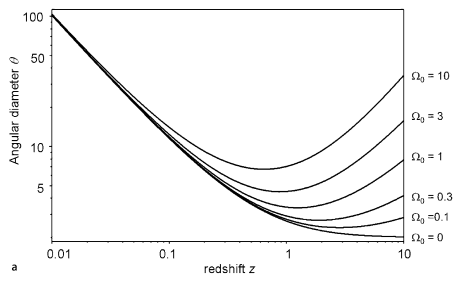
\includegraphics[scale=0.40]{angular_diameter78a_pp235Malcolm.png}
            \caption{\footnotesize{Variación del diámetro angular de una barra rígida de unidad de longitud propia para un desplazamiento al rojo dado con $\Omega_{\Lambda}=0$.}}
            %\label{fig:figura1}
    \end{minipage}
        \hspace{0.5cm}
    \begin{minipage}[b]{0.45\linewidth}
        \centering
            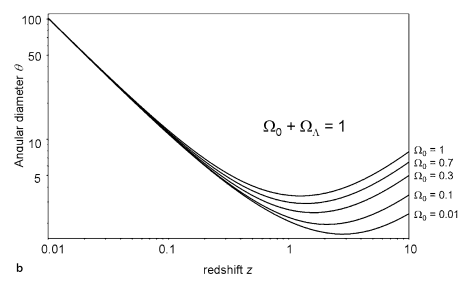
\includegraphics[scale=0.40]{angular_diameter78b_pp235Malcolm.png}
            
            \caption{\footnotesize{Variación del diámetro angular de una barra rígida de unidad de longitud propia para un $z$ dado con $\Omega_{\Lambda} \neq 0$, incluyendo el caso de geometría plana $\Omega_{\Lambda} + \Omega_0 =1$. }}
        %\label{fig:figura2}
    \end{minipage}
\end{figure}
    
    
    \subsubsection{Relación Densidad de Flujo – Desplazamiento al Rojo}

\begin{itemize} 

\item Modelos con $\Omega_{\Lambda} =0$:

Regresando a la sección 2.4,  habíamos encontramos una relación para la densidad de flujo de la fuente, esto es, la energía recibida por unidad de tiempo, por unidad de área y por unidad de ancho de banda, ec. (2.28)

\begin{equation}
	S(\nu_0) = \frac{N(\nu_1)h \nu_0 \Delta \Omega}{4 \pi \Delta t_0 \Delta \nu_0 (\pi/4) \Delta l^2},
\end{equation}

donde al haberse considerado la dilatación del tiempo cosmológico,  (2.7), las relaciones (2.8) y de la luminosidad, (2.22) se llegó a 

\begin{equation}
	S(\nu_0) = \frac{L(\nu_1) a(t_1)}{4 \pi D^2} = \frac{L(\nu_1) }{4 \pi D^2(1+Z)}.
\end{equation}

Para espectros que siguen la forma de ley de potencia $L(\nu) \propto \nu^{-\alpha}$ 

\begin{equation}
	S(\nu_0) = \frac{L(\nu_0) }{4 \pi D^2(1+Z)^{1+\alpha}},
\end{equation}


donde la medida de distancia $D$ es la determinada en (4.67), siendo la expresión para un Universo con $\Omega_0 > 0$, además de $\Omega_{\Lambda} =0$. La figuras 14 y 15 muestra la variación de la densidad de una fuente de luminosidad $1 \mathrm{W \, Hz^{-1}}$ con un espectro de potencia $L(\nu) \propto \nu^{-1}$ ($c/H_0 =1$)  para diferentes valores del parámero $\Omega_0$. 



\item $\Omega_{\Lambda} \neq 0$:

Así mismo, la figura 15 muestra la variación para modelos con valores finitos de $\Omega_{\Lambda}$ y geometría plana. 

Elegir el índice espectral $\alpha = 1$  en (4.72) implica que también hay variaciones en la densidad de flujo bolométrico (ver ecs. 2.31 y 2.33). Para el caso de galaxias, debe incluirse el espectro detallado de las mismas, lo cual se resuelve con las Correcciones K, mostradas en las relaciones (2.37,38,39). 

\end{itemize}

\begin{figure}[H]
        \begin{minipage}[b]{0.41\linewidth}
        %\centering
            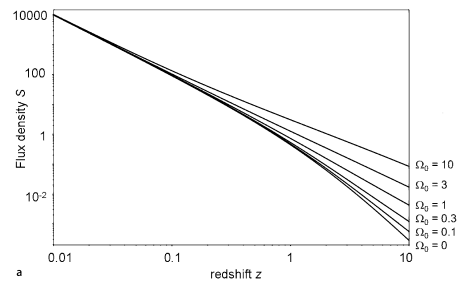
\includegraphics[scale=0.40]{79a_Malcolmpp237.png}
            \caption{\footnotesize{Modelos de mundo con $\Omega_{\Lambda}=0$.}}
            %\label{fig:figura1}
    \end{minipage}
        \hspace{0.9cm}
    \begin{minipage}[b]{0.36\linewidth}
        %\centering
            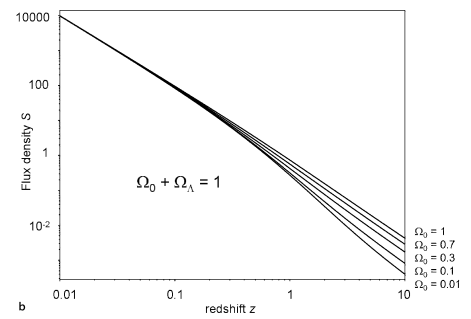
\includegraphics[scale=0.39]{79b_Malcolmpp237.png}
            
            \caption{\footnotesize{Modelos de mundo con $\Omega_{\Lambda} \neq 0$, incluyendo el caso de geometría plana $\Omega_{\Lambda} + \Omega_0 =1$. }}
        %\label{fig:figura2}
    \end{minipage}
\end{figure}

\vspace{0.4cm}
    
    
{\bf{\large{Imágenes Fantasmas}}}

Las {\textit{imágenes fantasmas}} son características en Modelos de Lema\^itre, los cuales presentan un $\dot{a} > 0$ además de secciones esféricas cerradas.

En el caso de modelos de mundo de Eddington – Lema\^itre, también con secciones esféricas, $\kappa >0$, la expansión casi se detiene a un desplazamiento al rojo crítico $z_c$, por esta razón hay tiempo para que las ondas electromagnéticas se propaguen desde la fuente hasta el observador un número de veces alrededor de la geometría cerrada del Universo. El objeto puede ser observado en direcciones opuestas o en la misma dirección en el cielo pero multiplicado, lo cual produce que sea observado en diferentes desplzamiento al rojo y por ende en distintos tiempos en su historia de vida.
    
    \begin{wrapfigure}[21]{r}{0.5\linewidth}                  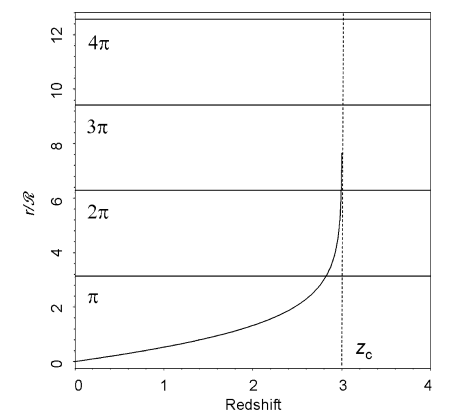
\includegraphics[width=0.65\textwidth]{710_Malcolmpp238.png}
        \caption{\footnotesize{$r/R'$ como una función del desplazamiento al rojo ($z$) para modelos de Eddington - Lema\^itre estacionarios en $z_c = 3$.}}
    \end{wrapfigure}

    De la sección de {\textit{dinámica de modelos de mundo con $\Omega_{\Lambda} \neq 0$}}, sec. 4.2, para estos modelos de  Eddington – Lema\^itre, el parámetro de densidad puede hallarse de la relación (4.46), siendo de $\Omega_0 = 1/27$ y el valor de $\Omega_{\Lambda}$ se obtiene de la relación (4.45,46), $\Omega_{\Lambda} = 32/27$. De esta manera, el radio de curvatura de la geometría cerrada viene siendo $R’ = (27/6)^{1/2} (c/H_0)$. Tomando estos valores e insertándolos en (4.64), una relación para $r/R’$ a un cierto $z$ es obtenida. Así, la figura 16 muestra esto para valores de $r/R’ = \pi, 2 \pi, 3 \pi, 4 \pi$. $r/R’ \rightarrow{\infty}$ a medida el desplazamiento al rojo estacionario vaya acercándose al valor $z_c=3$. 
    
    \newpage
    
    De la sección de {\textit{diámetros angulares}}, 2.3, la distancia medida se definió como:

\begin{equation}
	D = R’ \sin(r/R’),
\end{equation}
    
    así, considerando un índice espectral $\alpha = 1$, definido por $S \propto \nu^{-2}$ es

\begin{equation}
	S \propto	\frac{1}{[R’ \sin(r/R’)]^2 (1+z)^2}.
\end{equation}
     
     De esta relación, el mínimo en la densidad de flujo -  desplazamiento al rojo ocurre en $r/R’= \pi/2$ y diverge en $\pi$ con $z= 2.825$. Así mismo, para valores de $\pi < r/R’ < 2 \pi \rightarrow{z = 2.9929}, \, \, 2 \pi < r/R’ < 3 \pi \rightarrow{z = 2.99967}$. Que exista una divergencia, e.g., en $r/R’ = \pi$ se debe a que estamos observando el punto {\textit{antipodal}} {\footnote{el punto antipodal en la superficie esférica es el punto diametralmente opuesto a este. En un círculo están separados $180^{\circ}$. }} en la geometría cerrada para nuestra propia ubicación en el Universo.
    
   Esa luz se podría pensar  la de una galaxia en el punto antipodal que se enfoca y recibiríamos en nuestra Galaxia en $z=0$ y que para $r/R’ = 2  \pi$ observamos pero en $z=2.9923$, y así hasta que $z \rightarrow{z_c}$.  

Recordemos que los modelos de Lema\^itre no alcanzan un estado estacionario sino que $\dot{a} > 0$. Estos modelos tienen que ser finamente ajustado para que imágenes fantasmas puedan ser observadas. 

    
    Para modelos de Friendmann con $\Omega_{\Lambda} =0$ el efecto de imágenes fantasmas no ocurre; en todos los que tienen geometría espacial cerrada $r/R’ \rightarrow{\pi/2}$ como $z \rightarrow{\infty}$, en donde $\pi/2$ corresponde a rayos de luz que se propagan desde una densidad de flujo mínimo a la Tierra, entonces la posibilidad de observar la misma fuente en direcciones opuestas o múltiples imágenes del mismo objeto y en la misma dirección no existe. 
    
    El interés de considerar este fenómeno es que si tales imágenes `fantasmas’ existiesen, implicaría que el Universo en algún tiempo pasado experimentó una larga fase cuasi-estacionaria. Esto se ha tratado de verificar usando catálogos de fuentes de radio extragalácticas, pero no ha dado resultados positivos. 



\subsubsection{Volumen Comóvil dentro del Desplazamiento al Rojo $z$}
    
    
    
    
    
    
    
    
    
    
    
\end{document}
